\chapter{Lezione 16/03}

Il problema delle espressioni regolari è che non hanno esplicitamente una congiunzione o intersezione.
Se avessi l'intersezione potrei scrivere \(\bigwedge_{i=0}^n F p_i\) come \(\bigcap_{i=1}^n \Sigma* p_i \Sigma^*\).

Non avendolo però è necessario scrivere un'espressione regolare per ogni ordine.

Questo è perché nei linguaggi regolari non c'è il complemento, e dunque non c'è l'intersezione, questo perché di base non è necessario.
Ciò comporta però che descrivere una proprietà che non è presente sia complicato.

Quindi vogliamo un linguaggio che si avvicini di più all'idea informale di proprietà, poiché è già difficile e inevitabilmente inesatto il processo di formalizzazione di un idea.
Se il linguaggio è più vicino all'idea informale, allora sarà più facile formalizzare correttamente l'idea informale, e dunque sarà più facile verificare che il sistema soddisfa la proprietà desiderata.

Passiamo quindi a un linguaggio logico. Inizialmente con il prim'ordine, per poi passare alla logica temporale, che cerca di nascondere all'interno di operatori logici dei pattern ricorrenti in logica del prim'ordine.

Quali sono gli ogetti che ci interessano? L'universo, o ogetti del discorso, sono le parole \(w: [0,n)\to \Sigma\) oppure \(w: \N \to \Sigma\).

Immaginiamo di voler esprimere la proprietà \qi{Prima o poi il sistema ha stampato ed è in attesa del nuovo input}.
Essendo una congiunzione di proprietà, il che però deve far si che gli elementi dell'alfabeto non sia da considerarsi come atomiche.
Dobbiamo considerare \(\Sigma = 2^{AP}\), con \(AP\) l'insieme delle proposizioni atomiche.

\todo{Espandi esepio con \(p\) e \(i\) print e idle}

Dunque i nostri modelli saranno essenzialmente \(w:\N \to 2^{AP}\), ovvero a ogni istante temporale associamo l'insieme di proposizioni atomiche vere in quel momento.

Vediamo dunque col prim'ordine possiamo esprimere queste proprietà.
Dobbiamo quindi avere \(w \models \phi\).

Per il prim'ordine avremo una grammatica di questo tipo, con \(p \in AP\):
\[\phi ::= p(x) \mid \neg \phi \mid \phi \land \phi \mid \phi \lor \phi\mid \forall x \phi \mid \exists x \phi\]

Normalmente una grammatica di questo tipo porterebbe a un problema indecidibile, ma se ci concentriamo su sole stringhe come modelli allora torna decidibile.

Vediamo dunque la semantica del prim'ordine. La definiremo in maniera composizionale, ovvero definendo la semantica di una proposizione atomica e come gli operatori logici modificano la semantica delle proposizioni atomiche.
In particolare ci serve un assegnamento \(\chi : \Var \to N\) che ci dice ogni variabile a quale istante temporale si riferisce.
\(w,\chi \models p(x)\) se \(p \in w(\chi(x))\). Con \(w(\chi(x))\) si intende l'elemento di \(w\) in posizione \(\chi(x)\), ovvero l'insieme di proposizioni atomiche vere in quel momento, e \(p \in w(\chi(x))\) significa che \(p\) è una di queste proposizioni atomiche vere in quel momento.

Prendiamo ad esempio la parola \(w = \emptyset \set{i} \set{i} \set{i} \emptyset \set{i,p}\). Allora con \(\chi = \set{x \to 3}\) avremo \(w,\chi \not\models p(x)\) poiché \(p \not\in w(3)\), mentre con \(\chi' = \set{x \to 5}\) si ha \(w,\chi' \models p(x)\) poiché \(p \in w(5)\).

Continuando la semantica, avremo che:
\(w,\chi \models \neg \phi\) se\(w,\chi \not\models \phi\).
\(w,\chi \models \phi_1 \land \phi_2\) se \(w,\chi \models \phi_1\) e \(w,\chi \models \phi_2\).
\(w,\chi \models \phi_1 \lor \phi_2\) se \(w,\chi \models \phi_1\) o \(w,\chi \models \phi_2\).
Questo chiude la semantica della parte proposizionale.

Ora per dare la semantica agli operatori quantificatori, diremo:
\(w,\chi \models \forall x.\phi\) se per ogni \(n \in \N\), \(w,\chi[x \to n] \models \phi\). Ovvero sostituendo a \(x\) ogni possibile istante temporale, la formula \(\phi\) è soddisfatta.
\(w,\chi \models \exists x.\phi\) se esiste \(n \in \N\) tale che \(w,\chi[x \to n] \models \phi\). Ovvero sostituendo a \(x\) almeno un istante temporale, la formula \(\phi\) è soddisfatta.

Vediamo come modellare una proprietà sul futuro. Tipo \(\exists x. i(x) \land p_2(x)\). Ad esempio questo può essere inteso come \qi{Prima o poi il sistema ha stampato ed è in attesa del nuovo input}.
Se invece voglio dire che non ha mai due processi in una sezione critica, allora posso scrivere \(\forall x. \neg (p_1(x) \land p_2(x))\).

Se invece voglio dire che infinitamente spesso valga la proprietà \(i\). Qui ho una difficoltà, perché mi serve poter esprimere una relazioni tra istanti temporali.
Ci serve quindi poter esprimere il concetto di \qi{dopo}, è necessario introdurre una relazione d'ordine tra istanti temporali.
Sintatticamente inroduciamo il simbolo \(\preceq\), la cui semantica è:
\(w,\chi \models x\preceq y\) se \(\chi(x) \leq \chi(y)\). In questo caso sono stati nettamente separati i simboli \(\preceq\) e \(\leq\) per evidenziare che il primo è un simbolo del linguaggio ogetto, mentre l'altro è l'ordine usuale dei numeri naturali.
Nella pratica useremo \(\leq\) anche nel linguaggio ogetto poiché sarà chiaro dal contesto se si tratta di un simbolo del linguaggio o dell'ordine usuale dei numeri naturali.

Per esprimere quindi che una proprietà \(i\) si verifica infinitamente spesso, possiamo scrivere \(\forall x. \exists y. x \leq y \land i(y)\).
Se voglio esprimere che arriva un punto dopo il quale sarò sempre in idle posso scrivere \(\exists x. \forall y. x \leq y \to i(y)\).

In generale però possiamo osservare che quando parliamo di proprietà temporali ci troviamo sempre in uno di questi due casi:
\begin{itemize}
  \item \qi{Prima o poi} \(p\) è vero, ovvero \(\exists y. x \leq y \land p(y)\)
  \item \qi{Dopo un certo punto} \(p\) è sempre vero, ovvero \(\exists x. \forall y. x \leq y \to p(y)\)
\end{itemize}

Ma allora possiamo costruire un linguaggio che abbia sintatticamente due operatori che esprimono esattamente questi due pattern ricorrenti come semantica.

\section{Linear Temporal Logic}

Introdotta da Pnueli nel 1979. In questa logica lasciamo implicito l'istante in cui si verifica una proprietà, ci penserà la semantica degli operatori a gestire questo aspetto.
La grammatica è la seguente, con \(p \in AP\):
\[\phi ::= p \mid \neg \phi \mid \phi \land \phi \mid \phi \lor \phi \mid F\phi \mid G\phi\]
Dove \(F\) è l'operatore \q{prima o poi} (o \q{eventually}, \q{future}) e \(G\) è l'operatore \q{dopo un certo punto} (o \q{always}, \q{globally}).

Ovviamente anche ora parleremo di proprietà della parole, ma ora a differenza del prim'ordine non useremo più un assegnamento. Invece, per la semantica, utilizzeremo un indice \(i\) che rappresenta l'istante temporale in cui stiamo valutando la formula, e di conseguenza da cui iniziamo a guardare nel futuro.

La semantica è la seguente:
\(w,i \models p\) se \(p \in w(i)\).
La semantica degli operatori proposizionali è identica.
Venendo ai nuovi operatori invece abbiamo:
\(w,i\models F\phi\) se \(\exists j \geq i \st w, j \models \phi\), ovvero se \(\exists j: j \geq i \land w,j\models\phi\).
\(w,i\models G\phi\) se \(\forall j \geq i , w, j \models \phi\), ovvero se \(\forall j: j \geq i \to w,j\models\phi\).
Con questa sintassi però non è possibile esprimere proprietà che mi descrivono \q{il passato}, come \(\exists x \st p_1(x) \land \forall y, y\leq \neg p_2(x)\).

Di conseguenza, alla sintassi nell'81 vennero sostituiti \(F\) e \(G\) con due operatori binari e dimostrato che con questa agginuta la logica temporale risulta essere equivalente al prim'ordine.
In particolare, la sintassi diventa:
\[\phi ::= p \mid \neg \phi \mid \phi \land \phi \mid \phi \lor \phi \mid \phi U \phi \mid R\phi\]
Dove \(U\) è l'operatore \q{until} e \(R\) è l'operatore \q{release}
Intuitivamente \(U\) esprime che una proprietà \(p\) è vera fino a quando non diventa vera una proprietà \(q\), mentre \(R\) esprime che una proprietà \(p\) è vera a meno che non diventa vera una proprietà \(q\).

Formalmente:
\(w,i \models \phi_1 U \phi_2\) se \(\exists j \geq i \st w,j\models \phi_2\) e \(\forall k: i \leq k < j \to w,k\models \phi_1\)
\(w,i \models R\phi_1 \phi_2\) se \(\forall j \geq i \st w,j\models \phi_2\) o \(\exists k: i \leq k < j \land w,k\models \phi_1\)

Possiamo notare che \(F\phi \equiv \top U \phi\) e che \(G\phi \equiv \bot R \phi\), quindi \(F\) e \(G\) sono esprimibili in termini di \(U\) e \(R\).

\chapter{Lezione 30/03}

LTL ci permette di esprimere praticamente tutto ciò che è esprimibile con le espressioni \(\omega\)-regolari, tranne cose come il counting.

Dire che una proprietà \(P\) è vera in posizioni pari (NON ESCLUSIVAMENTE SUI PARI) si può fare facilmente con \({((\Sigma\Sigma)*(p\Sigma))}^\omega\) ma non è possibile esprimere questa proprietà in LTL, come neanche in prim'ordine.

Comunque in entrambe le sintassi manca anche l'operatore di next, che però ha senso solo se si parla di modelli con tempo discreto, e con modelli con tempo continuo non è detto che abbia senso.

Tale operatore è espresso come \(X \phi\), e la sua semantica è \(w,i \models X\phi\) se \(w,i+1 \models \phi\).

Grazie a questo operatore possiamo dire cose come \(G(p\land X \neg p)\), che può sembrare descriva la proprietà di essere vero solo in posizioni pari.

Ma andando a sviluppare questa formula, otteniamo:
\[w,0\models G(p\land X \neg p) \iff \forall j \geq 0, w,j \models (p\land X \neg p) \iff \forall j \geq 0, (w,j \models p \land w,j+1 \models \neg p)\]

Che è chiaramente insoddisfacibile. Il problema è che questa formula pretende che \(p\) sia vero in ogni punto.
Un modo più corretto per esprimere questa proprietà è \(G((p \leftrightarrow X \neg p) )\). Ad essere precisi questa ci dice che \(p\) è vera o solo sui pari o solo sui dispari. Per ottenere la proprietà che \(p\) è vera sui pari e falsa sui dispari, allora basta innescarla con \(p\) all'inizio, ovvero \(p \land G((p \leftrightarrow X \neg p) )\).

Espandendola abbiamo:
\[w,0 \models p \land G((p \leftrightarrow X \neg p) )\iff w,0 \models p \text{ e } \forall j \geq 0, w,j \models p \iff w,j+1 \models X \neg p\]

In questo modo abbiamo che \(p\) è vera in \(0\), allora deve essere falsa in \(1\), allora deve essere vera in \(2\), e così via, ottenendo la proprietà desiderata.

Questa però ci dice che la proprietà è soddisfatta solo in posizioni pari, non che è soddisfatta almeno in posizione pari, che abbiamo già detto non è esprimibile in LTL\@.

Dobbiamo ora dare una nozione formale al meta livello di equivalenza tra formule.

Ad esempio abbiamo che \(\land\) e \(\lor\) rispettano le leggi di De Morgan.

Inoltre abbiamo che \(U\) e \(R\) sono duali, infatti \(w,i \models \phi_1 U \phi_2\) se e solo se \(w,i \models \neg (\neg \phi_1 R \neg \phi_2)\).

Andiamo a dimostrare questa equivalenza:

\[w,i\models \phi_1 U \phi_2 \iff \exists j \geq i( w,j \models \phi_2 \land \forall i\leq k < j, w,k\models \phi_1)\iff\]
\[\iff \neg \neg \exists j \geq i\st( w,j \models \phi_2 \land \forall i\leq k < j, w,k\models \phi_1) \iff\]
\[\iff \neg \forall j \geq i,\neg( w,j \models \phi_2 \land \forall i\leq k < j, w,k\models \phi_1) \iff\]
\[\iff \neg \forall j \geq i, w,j \models \neg \phi_2 \lor \neg \forall i\leq k < j, w,k\models \phi_1 \iff\]
\[\iff \neg \forall j \geq i, w,j \models \neg \phi_2 \lor \exists i \leq k < j\st w,k\models \neg \phi_1 \iff\]
\[\iff w,i \models \neg (\neg \phi_1 R \neg \phi_2)\]

Ovviamente per essere un equivalenza stiamo dicendo che tutti questi i passaggi siano corretti a prescindere da \(w\) e \(i\).
In questo caso in effetti non abbiamo usato nulla di specifico su \(w\) e \(i\), e quindi indipendentemente dalla scelta dalla parola e dal punto in cui partiamo, questa equivalenza è sempre vera.

\begin{definition}{Equivalenza tra formule}
  Diremo che due formule \(\phi\) e \(\psi\) sono equivalenti, e scriveremo \(\phi \equiv \psi\), se per ogni parola \(w\) e ogni punto \(i\) si ha che \(w,i \models \phi\) se e solo se \(w,i \models \psi\).
\end{definition}

Grazie a questa definizione possiamo mostrare come LTL del 71 sia sussunta da quella dell'81, infatti \(F\phi \equiv \top U \phi\) e \(G\phi \equiv \bot R \phi\), dove \(\top\) e \(\bot\) sono simboli sintattici assunti presenti nella grammatica, con semantica \(w,i \models \top\) sempre vero e \(w,i \models \bot\) sempre falso. Questo era facile da intuire, poiché la semantica di \(F\) e \(G\) è parte di quella di \(U\) e \(R\), che non fanno altro che aggiungere ulteriori vincoli, i quali vengono ignorati se si usano \(\top\) e \(\bot\). Ovviamente questo mostra una proprietà di dualità tra \(F\) e \(G\), che è la stessa dualità tra \(U\) e \(R\).

Molto spesso, comunque, quello che mi interessa non è usare il counting, quindi il fatto che LTL non sia in grado di esprimere proprietà di counting non è un grosso problema. Inoltre, l'operatore \(X\) non è qualcosa di assoluto, poiché dipende dalla granularità della discretizzazione del tempo. Molto spesso a livello di proprietà pratiche non si usa proprio.

Omettendolo ottengo il frammento stattering free di LTL, che non è espressivamente equivalente a LTL intero, poichè non è possibile distinguere tra parole in cui c'è \qi{idle} in una posizione. Ad esempio le due parole \(ppp\neg p \neg p pp\) e \(p\neg p p\) sono indistinguibili in questo frammento, ma distinguibili in LTL\@. In un certo senso non importa \qi{quanto tempo} sto in uno stato, ma solo i cambiamenti di stato. La cosa importante di questa cosa è che questo operatore porta quasi sempre ad un aumento della complessità da \(NP\) a \(PSPACE\), quindi è un operatore che è meglio evitare se non è necessario.

Proprietà di one-step unfolding. Si può facilmente vedere che vale \(F\phi\equiv \phi \lor X F \phi\). Ho preso la mia formula e l'ho \qi{srotolata} di un passo. In teoria posso srotolarla di un numero qualsiasi di passi, ma srotolarla di un passo è sufficiente per poter costruire un automa. Vale lo stesso per \(G\phi\equiv\phi\land XG\phi\). Dunque saranno vere le opportune generalizzazioni per \(U\) e \(R\). In particolare

\[\phi_1 U \phi_2 \equiv \phi_2 \lor (\phi_1 \land X(\phi_1 U \phi_2 ))\]
\[\phi_1 R \phi_2 \equiv \phi_2 \land (\phi_1 \lor X(\phi_1 R \phi_2 ))\]

NNF ugale a logica classica usando dualità tra \(U\) e \(R\) e tra \(F\) e \(G\). Per quanto riguarda \(X\) invece, è un operatore self-dual, ovvero \(\neg X \phi \equiv X \neg \phi\).

Scrivi algoritmo formale (banale).

\begin{definition}{Lunghezza}
  la lunghezza di una formula \(\phi\) è una funzione che rispetta le seguenti regole:
  \begin{itemize}
    \item \(len(p) = 1\) per \(p \in AP\)
    \item \(len(Op \phi) = 1 + len(\phi)\) per \(Op \in \set{\neg,X}\)
    \item \(len(\phi_1 Op \phi_2) = 1 + len(\phi_1) + len(\phi_2)\) per \(Op \in \set{\land, \lor, U, R}\)
  \end{itemize}
\end{definition}

Chiaramente alla peggio portare in NNF mi raddoppia la lunghezza della formula, quindi se la formula originale è di lunghezza \(n\) allora la formula in NNF è di lunghezza al più \(2n\). Questo perché il peggior caso e qullo in cui abbiamo \(\neg\) come opertaore più esterno e tutti i letterali positivi. In questo caso infatti considerando l'albero sintattico andiamo a togliere il nodo in radice e aggiungere un nodo per ogni foglia. Essendo che il numero di foglie è lineare rispetto alla lunghezza della formula, allora la lunghezza della formula in NNF è al più \(2n\).

Vediamo ora qualche esempio di proprietà espressa di modellazione di sistema espressa in LTL\@.

\paragraph{Reachability}

Classicamente basta \(F\phi\), nel senso che nel mio modello voglio raggiungere uno stato in cui \(\phi\) è vera, e dunque basta dire che prima o poi \(\phi\) è vera. In maniera più strutturata, possiamo esprimerle come \(\phi_1 U \phi_2\), in cui non solo voglio raggiungere uno stato in cui \(\phi_2\) è vera, ma voglio anche che fino a quel momento il sistema si comporti in un certo modo, ovvero che \(\phi_1\) sia vera.

\paragraph{Safety}
Queste invece sono esprimibili con \(G\phi\), dove \(\phi\) è una formula che esprime la proprietà di sicurezza, ovvero che non accada qualcosa che non voglio che accada. Anche qui, dualmente, posso esprimerla con \(R\), ad esempio \(\phi_1 R \phi_2\) esprime che \(\phi_2\) è sempre vera a meno che non diventa vera \(\phi_1\), ovvero voglio dire non fare mai qualcosa di sbagliato a meno che non sia successo qualcosa che mi dice che non è più un problema, ad esempio un processo è terminato.

La cosa non è così semplice però, perché come abbiamo già visto, è possibile avere delle tracce spurie, ovvero percorsi nel grafo di computazione che sono ammesse solo perché nell'astrazione del modello si è perso qualche dettaglio, ma che in realtà non sono percorsi realizzabili nel sistema concreto.

Se voglio esprimere una proprietà una proprietà che voglio sia vera infinitamente spesso posso usare \(G F \phi\).

In questo modo posso filtrare tracce che non rispettano un vincolo di fairness. Una proprietà di \(G F \phi \to \psi\) è detta di strong fairness.

I problemi di decisione si basano sul modello di computazione, che abbiamo formalizzato tramite una struttura di kirpke \(K\) il cui linguaggio \(L(K)\) è l'insieme di tutte le parole che rappresentano esecuzioni del sistema concreto. Ora, dato un formula \(\phi\) di LTL\@, vogliamo decidere se \(K \models \phi\), ovvero se tutte le parole in \(L(K)\) soddisfano \(\phi\). Quindi se definiamo il linguaggio \(L(\phi) = \set{w \st w,0 \models \phi}\), allora il problema di verifica è decidere se \(L(K) \subseteq L(\phi)\).\footnote{Per brevità se sto iniziando da indice \(0\), posso scrivere \(w,0\models \phi\) come \(w\models \phi\).}

La negazione di questa proprietà è \(L(K) \cap \overline{L(\phi)} \neq \emptyset\), ovvero \(L(K) \cap L(\neg \phi) \neq \emptyset\). Quindi se un comportamento del sistema soddisfa la negata dalla formula, ho trovato un controesempio. Determinare se dato un sistema \(K\) esiste un suo comportamento che soddisfa la negata è il problema di model checking.

\chapter{Lezione 8/04}

Appunti mancanti per computer scarico, recuperare tramite registrazione audio e appunti fabrizio presenti in \lstinline{_files/_raw/Lezione_ASV_8_aprile_FABRIZIO}

\chapter{Lezione 13/04}

Problema dell'interezione di automi di Büchi.
L'esempio classico è il linguaggio \(L=a^\omega\).

Posso costruire due automi di due stati che accettano \(L\) uno che accetta nel primo stato e l'altro nel secondo.
Entrambi accettano \(L\), perché basta passare infinitamente spesso per uno stato accettante.
Ci aspetteremo quindi che l'interezioni degli automi accetti l'intersezione dei linguaggi, ovvero \(L\).
Ma creando l'automa intersezione tramite prodotto cartesiano, otteniamo un automa che non accetta alcuna parola.

Questo perché gli stati accettanti dell'automa intersezione sono quelli in cui entrambi gli automi originali sono in uno stato accettante, ma tali stati non sono raggiungibili.
Quello che si fa è ammettere che l'accettazione possa avvenire in modo asincrono, ovvero si creano due copie dell'automa intersezione, in cui in una copia si considerano accetanti gli stati in cui il primo automa è in uno stato accettante, e nell'altra copia si considerano accettanti gli stati in cui il secondo automa è in uno stato accettante, e poi si aggiungono delle transizioni che permettono di passare da una copia all'altra, in modo che una volta che il primo automa è passato per uno stato accettante, allora si passa alla copia in cui si considerano accettanti gli stati in cui il secondo automa è in uno stato accettante, e così via, in modo che se una parola è accettata da entrambi gli automi originali, allora è accettata anche dall'automa intersezione.

Formalmente, l'intersezione di automi di Büchi è
\[A_1 \Cap A_2 = \langle\Sigma, Q_1 \times Q_2\times\set{1,2}, \delta', Q_1^0 \times Q_2^0\times\set{1}, F_1 \times Q_2\times\set{1}\cup Q_1\times F_2\times\set{2} \rangle \]

con \(\delta'\) definita come segue:

\[\delta'((q_1,q_2,i),\sigma)=\delta_1(q_1,\sigma)\times\delta_2(q_2,\sigma)\times\begin{cases}
    \set{i}   & ,q_i\notin F_i \\
    \set{3-i} & ,q_i\in F_i
  \end{cases}\]

Quindi gli automi di Büchi sono chiusi per intersezione oltre che per unione. Vedremo successivamente che sono chiusi anche per complementazione, ma non sono chiusi per determinizzazione, ovvero non esiste una procedura per costruire un automa di Büchi deterministico equivalente a un automa di Büchi non deterministico.

Prendiamo ad esempio il linguaggio \(L = \Sigma^* 1^\omega\), con \(\Sigma= \set{0,1}\). In altre parole parole che iniziano in qualsiasi modo ma finiscono con soli \(1\). Possiamo facilmente riconoscere questo linguaggio con il seguente automa di Büchi non deterministico:
\todo{Aggiungi immagine}

Si potrebbe pensare di applicare la costruzione tramite sott'insiemi degli automi a stati finiti per provare a costruire un automa di Büchi deterministico equivalente, ma otterrei il seguente automa:
\todo{Aggiungi immagine}

Chiaramente questo automa, indipendentemente da come definiamo chi siano gli stati accettanti, verranno accettate parole che contengono un numero finito di \(0\), che non sono parole di \(L\).

Si potrebbe pensare quindi che il problema sia nel fatto di aver usato la costruzione tramite sott'insiemi e che esista un'altra procedura per costruire un automa di Büchi deterministico equivalente a un automa di Büchi non deterministico. Questo non è così.

\begin{proof}
  Supponiamo per assurdo che esista un DBA \(D\) tale che \(\mathcal{L}(D)=\mathcal{A} = \Sigma^* 1^\omega\)
  Allora
  \[w_0 = 1^\omega \in \mathcal{L}(D) \implies \exists r_0 \in Q^\omega \text{ run su } w_0 \text{ con } inf(r_0) \cap F \neq \emptyset\]

  Per raggiungere lo stato finale deve esistere un \(q_f \in r_0\) tale che \(q_f \in F\) e \(r_0=r_0' q_f r_0''\).
  Essendo però \(\delta_D\) deterministica, allora la parola sarà del tipo \(w_0=w_0'1w_0''\).

  Andiamo a costruire quindi una parola \(w_1\) tale che dopo l'\(1\) che porta il run ad avere \(q_f\) ha uno \(0\). Ovvero \(w_1 = w_0' 1 0 w_1\).

  Per essere accetata il run corrispondente deve avere.
  \todo{completa da registrazioni}
\end{proof}

AUTOMI GENERALIZZATI DI BÜCHI

L'idea è la stessa di quelli di Büchi classici, ma al posto di avere un unica condizione di accettazione, ne ha più di una.

Struttralmente quindi sarà:

\[A = \langle\Sigma,Q,\delta,Q_0,\langle F_0, \ldots,F_t\rangle\rangle\]
Ovvero al posto di avere un unico insieme di stati accettanti, abbiamo una tupla di insiemi di stati accettanti, e diremo che il linguaggio accettato da questo automa è
\[L(A)= \set{w\in\Sigma^\omega}[inf(r) \cap F_i \neq \emptyset, \forall i \in \set{0,\ldots,t}]\]

Tali automi sono stati introdotti solo per semplicità di trattazione, in quanto non sono più espressivi di quelli di Büchi classici.

In particolare possiamo usare la costruzione di intersezione asincrona che abbiamo visto precedentemente, ma essendo che gli stati sono identici, al posto di avere una copia per ogni automa che stiamo intersecando avremo una copia per ogni insieme di stati finali della tupla. In particolare avremo

\[\hat{A} = \langle\Sigma, \hat{Q},\hat{\delta},\hat{Q_0},\hat{F}\rangle\]
Con \(\hat{Q}=Q\times\set{0,\ldots,t}\), \(\hat{Q_0}=Q_0\times\set{0}\), \(\hat{F}=F_0\times\set{0}\) e la funzione di transizione definita come segue:

\[\hat{\delta}((q,i),\sigma) = \delta(q,\sigma) \times \begin{cases}
    \set{i}                & ,q\notin F_i \\
    \set{(i+1) \mod (t+1)} & ,q\in F_i
  \end{cases}\]

Tale \(\hat{\delta}\) fa in modo che all'arrivo in uno stato accettante di \(F_i\) si passi ad una copia diversa. Di conseguenza, essendo che una parola è accettata se e solo se il run corrispondente visita infinitamente spesso stati accettanti, per tornare infinitamente spesso in stati accettanti di \(F_0\) devo passare per tutte le copie, ovvero per stati accettanti di tutti gli insiemi \(F_i\), e dunque la parola è accettata se e solo se è accettata da tutti gli automi di Büchi classici che hanno come stati accettanti i diversi \(F_i\).

\begin{theorem}{}
  \[\forall \psi \in LTL, \exists A_\psi = \langle 2^{AP}, Q, \delta,Q_0,F\rangle \in NBA \st \mathcal{L}(\psi) = \mathcal{L}(A_\psi)\]
\end{theorem}

Prima di poter dimostrare questa cosa dobbiamo intodurre dei concetti.

\begin{definition}{Chiusura di una formula LTL}
  La chiusura di una formula LTL è una funzione \(cl:LTL\to 2^{LTL}\) tale che:
  \begin{enumerate}
    \item \(\phi \in cl(\phi)\)
    \item \(Op\phi'\in cl(\phi)\implies \phi'\in cl(\phi), \forall Op \in \set{\neg,X}\)
    \item \(\phi_1 Op \phi_2 \in cl(\phi) \implies \phi_1, \phi_2 \in cl(\phi), \forall Op \in \set{\land,\lor}\)
    \item \(\phi_1 U \phi_2 \in cl(\phi) \implies \phi_2 \lor (\phi_1 \land X(\phi_1 U \phi_2)) \in cl(\phi)\)
    \item \(\phi_1 R \phi_2 \in cl(\phi) \implies \phi_2 \land (\phi_1 \lor X(\phi_1 R \phi_2)) \in cl(\phi)\)
  \end{enumerate}
\end{definition}

\begin{example}{}
  Sia \(\phi=p\land X(rUq)\).
  La chiusura avrà i seguenti elementi:
  \begin{itemize}
    \item \(p\land X(rUq)\) per la regola 1
    \item \(p\) e \(X(rUq)\) per la regola 3
    \item \(rUq\) per la regola 2
    \item \(q \lor (r \land X(rUq))\) per la regola 4
    \item \(q\) per la regola 3
    \item \(r \land X(rUq)\) per la regola 3
    \item \(r\) per la regola 3
    \item \(X(rUq)\) per la regola 2
  \end{itemize}

  Questo esempio ci fa notare che le regole 4 e 5 portano ad aggiungere anche formule similmente alla regola 2.

  Si può facilmente vedere che \(2\abs{\phi}\geq \abs{cl(\phi)}\).
\end{example}

La chiusura è una nozione puramente sintattica, infatti tratta ugualmente cose come \(\land\) e \(\lor\). Di fatto la chiusura non è altro che l'insieme delle sottoforumle con l'aggiunta del one-step unfolding per \(U\) e \(R\).

\begin{definition}{Atomi di formule LTL}
  Data una formual \(\phi\) definiamo gli atomi di \(\phi\) come l'insime \(ATM(\phi)\subseteq 2^{cl(\phi)}\) tale che, un certo \(A \in ATM(\phi)\) se e solo se:
  \begin{itemize}
    \item \(A\subseteq cl(nnf(\phi))\)
    \item \(\forall p \in AP, p\in A \oplus  \neg p \in A\), ovvero \(p\in A\iff \neg p \notin A\)
    \item \(\phi_1 \land \phi_2 \in A \implies \phi_1, \phi_2 \in A\)
    \item \(\phi_1 \lor \phi_2 \in A \implies \phi_1 \in A \text{ o } \phi_2 \in A\)
    \item \(\phi_1 R \phi_2 \in A \implies \phi_2 \land (\phi_1 \lor X(\phi_1 R \phi_2)) \in A\)
    \item \(\phi_1 U \phi_2 \in A \implies \phi_2 \lor (\phi_1 \land X(\phi_1 U \phi_2)) \in A\)
  \end{itemize}
\end{definition}

Notare che l'operatore \(X\) non è presente nelle condizioni dell'atomo, questo perché la semantica di \(X\) necessità di parlare di più punti della parola, e dunque non è possibile definire una condizione che riguarda solo un punto della parola, come invece è possibile fare per gli altri operatori.

\begin{definition}{Sequenza di Hintikka}
  Una sequenza di Hintikka per una formula \(\phi\) è una parola infinita di atomi di \(\phi\) ovvero \(\alpha \in (ATM(\phi))^\omega\) tale che:
  \begin{enumerate}
    \item \(\phi \in \alpha_0\)
    \item \(\forall i, X\phi' \in \alpha_i \implies \phi' \in \alpha_{i+1}\)
    \item \(\forall i, \phi_1U\phi_2 \in \alpha_i \implies \exists j \in \N\st\phi_2\in\alpha_{i+j}\)
  \end{enumerate}
\end{definition}

\begin{theorem}{}
  \[\forall \phi \in LTL, Sat(\phi) \iff \exists \alpha \in (ATM(\phi))^\omega\st\alpha \text{ è una sequenza di Hintikka per } \phi\]
\end{theorem}
\begin{proof}
  VEDI REGISTRAZIONE
\end{proof}

Possiamo finalmente dimostrare il teorema di traduzione da LTL a NBA\@.
Per fare ciò anremo a costruire un automa di Büchi \(A_\phi\) che accetta esattamente le sequenze di Hintikka per \(\phi\), e dunque, essendo che una parola soddisfa \(\phi\) se e solo se esiste una sequenza di Hintikka per \(\phi\) che è uguale alla parola, allora \(A_\phi\) accetterà esattamente le parole che soddisfano \(\phi\).

Sia quindi \[A_\phi = \langle 2^{AP}, Q, \delta, Q_0, \hat{F} = \langle F_0, \ldots, F_t\rangle\rangle\]
Dove \(Q = ATM(\phi)\), \(Q_0 = \set{A \in ATM(\phi) }[\phi \in A]\), la funzione di transizione \(\delta\) si assicurerà che varrà la seconda condizione delle sequenze di Hintikka, ovvero
\[\delta(A,\sigma)=\begin{cases}
    \set{A'\in ATM(\phi)}[\forall X\psi \in A, \psi \in A'] & , \sigma = A \cap AP \\
    \emptyset                                               & , \text{ altrimenti}
  \end{cases}\]
mentre gli stati di accettazione saranno quelli che soddisfano la terza condizione delle sequenze di Hintikka, creando un insieme di stati di accettazione per ogni formula del tipo \(\phi_1 U \phi_2\) presente nella chiusura, ovvero
\[\hat{F} = \set{\set{A\in ATM(\phi)}[\phi_1 U \phi_2 \in A \implies \phi_2\in A]}[\phi_1 U \phi_2 \in cl(\phi)]\]

Tale costruzione ci permette di accettare solo parole che passano infinitamente spesso per stati in cui ogni until è soddisfatto localmente, ovvero \(\phi_1 U \phi_2\) è vera perché \(\phi_2\) è vera.


\begin{example}{}
  Sia \(\phi= F p \land q U r\).
  \[cl(\phi) = \set{\phi, Fp,qUr, r\lor q \land X(q\cup r),p\lor XFp, r,p,q,X(qUr),xFp}\]

  Fortunatamente non tutte le combinazioni di questi elementi sono atomi validi.
  Possiamo partire dagli stati iniziali, ovvero dagli atomi che contengono \(\phi\),

  INSERIRE IMMAGINI ATOMI
\end{example}

\chapter{Lezione 20/04}

A questo punto dobbiamo capire come usare questi automi per risolvere problemi di model checking e soddisfacibilità.

In particolare, data una struttura di kripke dobbiamo capire se questa soddisfa una formula \(\psi\). Questo equivale a dire che
\(\mathcal{L}(k)\subseteq \mathcal{L}(\psi) = \mathcal{A_\psi}\). Questo però equivale a richiedere che tutti i percorsi di \(k\) siano accettati da \(\mathcal{A_\psi}\).

Per semplicità, piuttosto di considerare che tutti i percorsi di \(k\) siano accettati da \(\mathcal{A_\psi}\), possiamo considerare il modello della negata e verificare che l'intersezione sia vuota.

Ricordiamo che la struttura di kripke \(k\) è definita come \(k = \langle W, R, AP, \lambda, w_0\rangle\) con \(W\) insieme dei mondi possibili o stati, \(R \subseteq W\times W\) relazione di transizione, \(AP\) insieme di proposizioni atomiche, \(\lambda: W \to 2^{AP}\) funzione di etichettatura che associa a ogni stato un insieme di proposizioni atomiche vere in quello stato, e \(w_0\) mondo iniziale.

A quel punto cotruire un automa risulta molto facile considerando \(A_k = \langle \Sigma=2^{AP}, Q = W, \delta, q_0 = w_0,  F=W\rangle\) con
\[\delta(w,\sigma) = \begin{cases}
    \set{w' \in W}[R(w,w')] & , \text{ se } \sigma = \lambda(w) \\
    \emptyset               & , \text{ altrimenti}
  \end{cases}\]

Tale automa accetta tutte e sole le parole del linguaggio della struttura di kripke \(k\), e dunque se l'intersezione di prima risulta essere \(\mathcal{L}(A_k) \cap \mathcal{L}(A_{\neg\psi})\), ovvero \(A_{k,\neg\psi} = A_{\neg\psi} \cap \mathcal{L}(A_k)\).
Quindi \(k\models \psi\) se e solo se \(A_{k,\neg\psi} = \emptyset\).

Questo va bene per il model checking, per la soddisfacibilità invece è sufficiente costruire \(A_\psi\) e verificare che \(\mathcal{L}(A_\psi)\neq \emptyset\). Per la validitò uguale ma usando \(A_{\neg\psi}\) e controllando che \(\mathcal{L}(A_{\neg\psi}) = \emptyset\).

Quindi l'ultima cosa che ci serve è un algoritmo per verificare se il linguaggio di un automa di Büchi è vuoto o meno.

Consideriamo per ora un NFA dato da \(A = \langle \Sigma,Q,\delta,Q_0,F\rangle\) e cerchiamo di capire se \(\mathcal{L}(A) = \emptyset\).

Consideriamo inizialmente l'esempio in figura.

\todo{Aggiungi immagine}

Intuitivamente per capire se è vuoto o meno dobbiamo vedere se esiste un percorso da uno stato iniziale a uno stato di accettazione, ovvero che uno stato finale sia raggiungibile dallo stato iniziale.

Trovato un percorso infatti posso sembre vedere quali archi abbiamo attraversato e usarne le etichette per sintetizzare la parola accettata.

Nel'esempio di prima \(S_0 S_1 S_2\) è un percorso accettante, le cui etichette sono \(bb\). Questo ci dice che \(bb\in \mathcal{L}(A)\).

Un modo banale è di usare un normale algoritmo di reachability sul grafo trasposto a partire dagli satati finali, e vedere se riesco a raggiungere uno stato iniziale, verificabile con un iterazione sugli stati raggiunti.

Esiste però un algoritmo non in NLOGSPACE, ovvero non deterministico a cui basta spazio logaritmico.

TODO PULISCI ALGORITMO E USA AMBIENTE APPROPRIATO

\begin{enumerate}
  \item Guess \(s \in Q_0\)
  \item Guess \(\sigma \in \Sigma\)
  \item Guess \(s' \in \delta(s,\sigma)\)
  \item If \(s' \in F\) then
  \item return yes
  \item else
  \item s \(\gets t\)
  \item goto 2
\end{enumerate}

Questo è non deterministico perché ci sono dei guess, valuiamo il perché è LOGSPACE\@.

Qui abbiamo 3 variabili \(s, \sigma, s'\) ma ognuna di queste può rappresentare un elemento di \(Q\) o \(\Sigma\) in spazio logaritmicol, in particolare \(2\log(\abs{Q}) + \log(\abs{\Sigma})\).

Sapendo che lo spazio è limitato, possiamo aggiungere la condizione di terminazione per la procedura contando il numero di archi attraversati, se supera il numero di stati sono in un ciclo sicuramente.

\begin{enumerate}
  \item count \(\gets 0\)
  \item Guess \(s \in Q_0\)
  \item Guess \(\sigma \in \Sigma\)
  \item Guess \(s' \in \delta(s,\sigma)\)
  \item If \(s' \in F\) then
  \item   return yes
  \item else if count < \(\abs{Q}\)
  \item   s \(\gets t\)
  \item goto 2
  \item else
  \item   return no
\end{enumerate}

Questa nuova variabile è ancora logaritmica.

Dobbiamo ora estendere agli automi di Büchi, in cui non voglio semplicemente raggiungere uno stato, ma voglio raggiungere uno stato infinite volte.

Possiamo estendere l'algoritmo precedente facendo guess dello stato da raggiungere, per potermelo ricordare, e poi verificando che ci ritorno.

\begin{enumerate}
  \item Guess \(s \in Q_0\)
  \item Guess \(\sigma \in \Sigma\), Guess \(s' \in \delta(s,\sigma)\)
  \item \(s'\gets t\)
  \item if \(s' \in F\) then
  \item   Guess \(\sigma \in \Sigma\), Guess \(s \in \delta(s',\sigma)\)
  \item   if \(s = s'\) then
  \item     return yes
  \item   else
  \item     goto 5
  \item else
  \item  goto 2
\end{enumerate}

Questo algoritmo è ancora in NLOGSPACE\@, e prima trova un percorso verso uno stato finale, e poi verifica che esiste un ciclo che torna a quello stato finale, dunque almeno un modo per passarci infinitamente spesso esiste.

Per farlo in maniera direttamente deterministica calcolando le componenti fortemente connesse del grafo, e verificando se esiste uno stato finale che è in una componente fortemente connessa. Di quelli che hanno questa proprietà, bisogna verificare che siano raggiungibili da uno stato iniziale, e se è così allora il linguaggio è non vuoto, altrimenti è vuoto.

Per gli automi di CO-Büchi invece, è sufficiente escludere i nodi di rifiuto nel calcolo delle componenti fortemente connesse, in modo da individuare cicli che non passano mai per stati di rifiuto, e verificare che tali cicli siano raggiungibili dallo stato iniziale, eventualmente passando anche per stati di rifiuto (poiché solo un numero finito di volte).

Andiamo quindi a dimostrare che con gli automi di Büchi accettano tutti e soli i linguaggi omega-regolari.

Partiamo dal teorema sugli automi a stati finiti.

\begin{theorem}
  Un linguaggio \(L\) è regolare se e solo se \(\exists NFA A \st \mathcal{L}(A) = L\)
\end{theorem}

Questo è facile da vedere ed è dato per scontato dal corso di EDIT.

\begin{theorem}
  Un linguaggio \(L\) è \(\omega-\)regolare se e solo se \(\exists NBA A \st \mathcal{L}(A) = L\)
\end{theorem}

\begin{proof}
  \begin{description}
    \item[(\(\implies\))] \(L\) \(\omega-\)regolare \(\implies \exists \gamma = \alpha_1\beta_1^\omega+\alpha_2\beta_2^\omega+\cdots + \alpha_n\beta_n^\omega \st \mathcal{L}(\gamma) = L\). Ovviamente ogni \(\alpha_i,\beta_i\) sono regolari, quindi dal teorema precedente esistono \(DFA A_{i}, B_{i}\) tali che \(\mathcal{L}(A_i) = \alpha_i\) e \(\mathcal{L}(B_i) = \beta_i\).
      Cotruiamo quindi per ogni componente \(i\) un automa di Büchi \(C_i= \langle \Sigma, Q_A \cup Q_B, \delta, \set{q_{0_A}}, \set{q_{0_B}}\rangle\) con \(\delta\) definita come:
      \[\delta(q,\sigma)=\begin{cases}
          \set{\delta_A(q,\sigma)}          & ,q \in Q_A \land \delta_A(q,\sigma)\notin F_A \\
          \set{\delta_A(q,\sigma), q_{0_B}} & ,q \in Q_A \land \delta_A(q,\sigma)\in F_A    \\
          \set{\delta_B(q,\sigma)}          & ,q \in Q_B \land \delta_B(q,\sigma)\notin F_B \\
          \set{\delta_B(q,\sigma), q_{0_B}} & ,q \in Q_B \land \delta_B(q,\sigma)\in F_B    \\
        \end{cases}\]

      Tale costruzione fa si che ogni componente si comporti come la parte regolare \(\alpha_i\), fino a non-deterministicamente decidere di passare alla parte regolare \(\beta_i\), che è estesa per essere un ciclo, in modo da passare infinitamente spesso per lo stato \(q_{0_B}\) che è l'unico stato accettante, e dunque accettare esattamente le parole di \(\alpha_i\beta_i^\omega\). A questo punto mi è sufficiente fare l'unione di tutti questi automi \(C_i\) per ottenere un automa di Büchi che accetta esattamente le parole di \(\gamma\), ovvero di \(L\).
    \item[(\(\impliedby\))] Consideriamo il NBA \(N = \langle \Sigma, Q, \delta, Q_0, F\rangle\) con \(F = \set{q_0\ldots,q_k}\) stati finali di \(N\). Per \(i \in \set{1,\ldots,k}\) definiamo \(A_i = \langle \Sigma, Q, \delta, Q_0, \set{q_i}\rangle\) e \(B_i = \langle \Sigma, Q, \delta, \set{q_i}, \set{q_i}\rangle\). Interpretando ognuno di questi automi come NFA otteniamo che i linguaggi accettati da \(A_i\) e \(B_i\) sono regolari per il teorema precedente. Inoltre, possiamo separare il nostro \(N\) in \(k\) sottoautomi, ognuno dei quali con \(F_i = \set{q_i}\). Ovviamente il linguaggo dell'unione di questi sottoautomi è uguale a quello di \(N\). Ognuno di questi sottoautomi però ha linguaggio \(L(N_i) = L(A_i)\cdot L(B_i)\omega\). Dunque \(L(N) = \bigcup_{i=1}^k L(A_i)\cdot {L(B_i)}^\omega\), ovvero è \(\omega-\)regolare.
  \end{description}
\end{proof}

Quindi i NBA sono sufficientemente espressivi per accettare tutti e soli i linguaggi \(\omega-\)regolari, a differenza di come abbiamo visto per LTL. Lo abbiamo osservato con l'esempio dell'espressione regolre  che accetta le parole che hanno P vera in posizione pari. Questo è facilisimo però da fare con un automa di Büchi, banalmente

P
->
SF  N
<-
*

Vediamo ora un elenco di diverse condizioni di accettazioni per automi che caratterizzano diversi tipi di linguaggi e proprietà di essi. Considerato \(\rho\) un run di un automa avremo:

\begin{itemize}
  \item Accettazione al finito, \(last(\rho) \in F\)
  \item Accettazione di Buchi, \(\inf(\rho) \cap F \neq \emptyset\) o CO-Buchi, \(\inf(\rho) \subseteq F = \emptyset\)
  \item Generalized Buchi, \(\bigwedge_i \inf(\rho) \cap F_i \neq \emptyset\) o Generalized CO-Buchi, \(\bigvee_i \inf(\rho) \cap F_i = \emptyset\)
  \item Accettazione di Muller, abbiamo \(F\subseteq 2^Q\), \(\inf(\rho) \in F\). Questa è più simile a quella a finito che alle altre, perché per accettare richiediamo una condizione specifica per il comportamento all'infinito, mentre in quelli di buchi è sufficiente che uno stato sia attraversato infinitamente spesso il resto non mi interessa. Questa è molto più costosa però, perché non mi basta usare raggiungibilità, ma devo verificare com'è fatto il run, e verificare se la sua parte infinita è in \(F\).
  \item Accettazione di Rabin, abbiamo \(F = {(2^Q\times 2^Q)}^*\), quindi \(F = \langle (G_i,B_i),\ldots,(G_k, B_k)\rangle\), \(\bigvee_i \inf(\rho) \cap G_i \neq \emptyset \land \inf(\rho) \cap B_i = \emptyset\)
  \item Accettazione di Street, abbiamo \(F = {(2^Q\times 2^Q)}^*\), quindi \(F = \langle (G_i,B_i),\ldots,(G_k, B_k)\rangle\), \(\bigwedge_i \inf(\rho) \cap G_i \neq \emptyset \lor \inf(\rho) \cap B_i = \emptyset\)
\end{itemize}

Le ultime 3 nel caso non deterministico si possono ridurre a quelle di Büchi, con un costo non indifferente, mentre per il determinismo non è possibile trovare una riduzione a quelle di Büchi, e dunque sono più espressive.

\chapter{Lezione 27/04}

Passiamo ora dalle logiche temporali lineari a quelle ramificate, in particolare con \(CTL^*\) (full computation tree logic) che contiene LTL ma permette di esprimere anche proprietà che non sono esprimibili in LTL\@.

In particolare vedremo il frammento \(CTL\), che è un sottoinsieme di \(CTL^*\) che però è più facile da verificare, di cui vorremo risolvere il model checking. In particolare vedremo inizialmente un algoritmo diretto per il model checking di \(CTL\), e poi vedremo un alogoritmo più efficiente che usa una struttura dati specifica chiamata OBDD\@.

In particolare questa logica aggiunge dei quantificatori sui percorsi, \(A\) e \(E\), che indicano rispettivamente che una proprietà è vera su tutti i percorsi o su almeno un percorso.

\begin{definition}{Grammatica \(CTL^*\)}
  La grammatica di \(CTL^*\) è formata da due grammatiche dette grammatica delle formule di stato \(\phi\) e grammatica delle formule di percorso\(\psi\), definite come segue:
  \[\phi ::= p \in AP \mid \neg \phi \mid \phi \land \phi \mid \phi \lor \phi \mid A\psi \mid E\psi\]
  \[\psi ::= \phi \mid \neg \psi \mid \psi \land \psi \mid \psi \lor \psi \mid X\psi \mid \psi U\psi \mid \psi R\psi\]

\end{definition}
Possiamo qundi vedere \(\psi\) come \(LTL\) su \(\phi\). Per la soddisfacibilità in \(LTL\) abbiamo detto che per \(\psi \in LTL\) \(k \models_{LTL} \psi\) se ogni percorso della struttura di kripke soddisfa la proprietà. Possiamo modellarlo anche in \(CTL^*\) con \(k \models_{CTL^*} A\psi\), ovvero \(\psi\) è vera su tutti i percorsi.

Passando alla semantica per \(\psi\) è praticamente a LTL se non per il caso atomico in cui va generalizzato da \(p\) a \(\phi\), mentre per la semantica per \(\phi\) è più complessa.

Per i casi base e per i connettivi booleani è abbastanza intuitiva, mentre per i quantificatori sui percorsi si ritorna a \(\psi\).

\begin{definition}{Semantica \(CTL^*\)}
  Data una struttura \(k = \langle AP, W, R, w_0, \lambda \rangle\) con \(AP\) insieme di proposizioni atomiche, \(W\) insieme dei mondi possibili o stati, \(R \subseteq W\times W\) relazione di transizione, \(w_0\) mondo iniziale e \(\lambda: W \to 2^{AP}\) funzione di etichettatura che associa a ogni stato un insieme di proposizioni atomiche vere in quello stato, e dato uno stato \(w \in W\) di partenza (\(w_0\) se omesso), diremo che:
  \begin{itemize}
    \item \(k,w \models p\) se e solo se \(p \in \lambda(w)\)
    \item \(k,w \models \neg \phi\) se e solo se \(k,w \not\models \phi\)
    \item \(k,w \models \phi_1 \land \phi_2\) se e solo se \(k,w \models \phi_1\) e \(k,w \models \phi_2\)
    \item \(k,w \models \phi_1 \lor \phi_2\) se e solo se \(k,w \models \phi_1\) o \(k,w \models \phi_2\)
    \item \(k,w \models A\psi\) se e solo se \(\forall \pi \in Paths(k,w), k,\pi \models \psi\)
    \item \(k,w \models E\psi\) se e solo se \(\exists \pi \in Paths(k,w), k,\pi \models \psi\)
  \end{itemize}
  Importante notare che fino ai quantificatori sui percorsi la semantica è definita su stati, quindi non ha alcuna nozionne temporale, mentre nei quantificatori si passa alla semantica LTL\@, che è definita sui percorsi, e dunque ha una nozione temporale. Normalmente a LTL basterebbe \(\pi\), ma essendo che in una formula di percorso posso tornare a una formula di stato è necessario mantenere la struttura \(k\) per poter valutare le formule di stato che possono essere presenti in \(\psi\).

  In particolare, per la semantica di \(\psi\) abbiamo esattamente la stessa semantica di LTL\@, con l'unica differenza che
  \[k, \pi, i\models \text{ se e solo se} k,{(\pi)}_i\models \phi\]
\end{definition}

Vedimo ora il frammento \(CTL\) di \(CTL^*\), che è un sottoinsieme di \(CTL^*\) in cui ogni operatore temporale è preceduto da un quantificatore sui percorsi.

Quello che cambia è la grammatica di \(\psi\), che non è l'intera grammatica di LTL\@, ma solo:
\[\psi ::= X\phi \mid \phi U\phi \mid \phi R\phi\]

In questo modo non c'è nesting di operatori temporali, e dunque ogni operatore temporale è preceduto da un quantificatore sui percorsi, e dunque ogni formula di percorso è del tipo \(X\phi\), \(\phi U \phi\) o \(\phi R \phi\).

Una formulazione alternativa e la prima proposta usa un'unica grammatica:
\[\phi ::= p \in AP \mid \neg \phi \mid \phi \land \phi \mid \phi \lor \phi \mid AX\phi \mid EX\phi \mid \phi AU \phi \mid \phi AR \phi \mid \phi EU \phi \mid \phi ER \phi\]

Questa sintassi esplicità è più prolissa ma è usata in molti software perché il problema di model checking di \(CTL\) è risolto risolvendo dei sottoproblemi per le sottoformule di questa forma e poi combinando.

Essendo molto prolissa, se ne utilizza una versione in cui si rimuovono quelli non necessari, ad esempio \(\land\) in presenza di \(\lor\) e \(\neg\).
Chiaramente questo vale per ogni coppia di operatore duale, ad esempio \(A\) e \(E\), \(U\) e \(R\), \(X\) e \(X\).

Dunque \(\neg AX\phi \equiv E\neg X \phi \equiv EX \neg \phi\), quindi l'operatore \(AX\) è ridondante.
Similmente \(\neg A \phi_1 U \phi_2 \equiv E \neg (\phi_1 U \phi_2) \equiv E \neg \phi_1 R \neg \phi_2\), e di conseguenza \(AU\) è ridondante. Ugualemente \(AR\) è ridondante. Quindi a livello algoritmico è sufficiente considerare solo il \q{frammento esistenzaile} di \(CTL\)\@, ovvero quello che contiene solo \(E\) come quantificatore.

Consideriamo inoltre, \(\phi_1 R \phi_2\). Supponiamo che \(\phi_1\) non sia mai vera, allora \(\phi_1 R \phi_2\) è vera se e solo se \(\phi_2\) è sempre vera, ovvero \(G\phi_2\). Altrimenti \(\phi_1\) dev'essere sempre vera fino a quando \(\phi_2\) non diventa vera, e dunque \(\phi_1 R \phi_2\) è vera se e solo se \(\phi_1 U \phi_2\). Dunque \(\phi_1 R \phi_2 \equiv G \phi_2 \lor \phi_2 U (\phi_1 \land \phi_2)\).

Formalmente \(\phi_1 R \phi_2\) è definita come:
\[\forall j \geq i, (\pi, j \models \phi_2 \lor \exists k \geq i, \pi, k \models \phi_1 \land \phi_2)\]

Il primo disgiunto è esattamente \(G\phi_2\), mentre il secondo disgiunto è esattamente \(\phi_2 U (\phi_1 \land \phi_2)\).
Questo vale a livello di LTL, ma a livello di \(CTL\) dobbiamo vederlo usando solo \(\lor\) e \(E\).
\[E \phi_1 R \phi_2 \equiv E(G\phi_2 \lor \phi_2 U(\phi_1 \land \phi_2))\]

Essendo che \(E\) distribuisce su \(\lor\) abbiamo proprio
\[E \phi_1 R \phi_2 \equiv E G\phi_2 \lor E \phi_2 U(\phi_1 \land \phi_2)\]

Dunque la logica che andremo veramente a risolvere è la seguente:
\[\phi::= p \in AP \mid \neg \phi \mid \phi \lor \phi \mid EX \phi \mid E\phi U \phi \mid EG \phi\]

Quello che andremo a fare è un algoritmo bottom-up, in cui risolviamo le sottoformule e andremo ad etichettare il nostro modello con delle etichette che indicano quali formule sono soddisfatte in ogni stato.

Prendiamo ad esempio \(E((p\land q) U r)\equiv E((\neg(\neg p \lor \neg q))U r)\). Andremo a etichettare ogni stato che soddisfa \(p\) con \(f_p\), ogni stato che soddisfa \(q\) con \(f_q\), ogni stato che soddisfa \(\neg p \lor \neg q\) con \(f_{\neg p \lor \neg q}\) e così via.

Prima di vedere l'algoritmo però ci serve ampliare il concetto di one-step unfolding visto in precedenza.
In particolare, \(\phi_1 U \phi_2 \equiv \phi_2 \lor (\phi_1 \land X(\phi_1 U \phi_2))\). In \(CTL^*\) quindi avremo
\[E(\phi_1 U \phi_2 )\equiv E(\phi_2 \lor (\phi_1 \land X(\phi_1 U \phi_2))) \equiv E\phi_2 \lor E(\phi_1 \land X(\phi_1 U \phi_2))\]

Nella sintassi di \(CTL\)\@, non possiamo esprimere \(E \phi_2\), ma quello che sta dicendo questa formula è che esista un percorso il cui primo stato soddisfa \(\phi_2\), che è equivalente a richiedere semplicemente \(\phi_2\).
Per quanto riguarda \(E(\phi_1 \land X(\phi_1 U \phi_2))\) stiamo richiedendo che esista un percorso in cui \(\phi_1\) è vero in radice e che lo stato successivo soddisfa \(\phi_1 U \phi_2\). Questo è equivalente a \(\phi_1 \land E(X (\phi_1 U \phi_2))\).
Quest'ultimo pezzo può essere riscritto come \(\phi_1 \land EX (E \phi_1 U \phi_2)\), e dunque abbiamo una formula in \(CTL\) per one-step unfolding.

Dobbiamo fare lo stesso con \(G\) e per farlo vedere passeremo per \(R\)
\[E(\phi_1 R \phi_2) \equiv E(\phi_2 \land (\phi_1 \lor X(\phi_1 R \phi_2)))\equiv\]
\[\phi_2 \land E(\phi_1 \lor X(\phi_1 R \phi_2))\equiv\]
\[\phi_2 \land (\phi_1 \lor EX (E \phi_1 R \phi_2))\]

Essendo che \(G \phi_2 \equiv \bot R \phi_2\), abbiamo che \(EG \phi_2 \equiv \phi_2 \land EX (EG \phi_2)\) sostituendo e semplificando \(\bot\).

Iniziamo quindi a vedere questi algoritmi partendo dal \(X\).

Iniziamo dalla definizione di chiusura, similmente a quella che abbiamo visto per LTL.

\(cl(\phi) \in NCTL\) è definita come
\begin{itemize}
  \item \(\phi \in cl(\phi)\)
  \item \(\neg \phi' \in cl(\phi)\implies \phi' \in cl(\phi)\)
  \item \(\phi_1 \lor \phi_2 \in cl(\phi)\implies \phi_1, \phi_2 \in cl(\phi)\)
  \item \(EX \phi' \in cl(\phi)\implies \phi' \in cl(\phi)\)
  \item \(E\phi_1 U \phi_2 \in cl(\phi)\implies \phi_1, \phi_2 \in cl(\phi)\)
  \item \(EG \phi' \in cl(\phi)\implies \phi' \in cl(\phi)\)
\end{itemize}

Quello che farà l'algoritmo è etichettare ogni stato con le formule di \(cl(\phi)\) che sono soddisfatte in quello stato andando bottom-up\@, ovvero partendo dalle formule proposizionali e risalendo fino alla formula \(\phi\) che vogliamo verificare.

Per \(EX\) l'algoritmo è il seguente\footnote{Il tipo \(Unit\) è il tipo che rappresenta l'assenza di un valore, è usato per indicare che la funzione non restituisce nulla di significativo, ma viene eseguita solo per i suoi effetti collaterali.}.

\begin{algorithmdesc}{Checking \(EX\)}
  \begin{algorithmic}[1]
    \Statex{} \textbf{signature} \(\textsc{CheckEX:} \quad Kripke \times Formula \to Unit\)
    \Function{\(\textsc{CheckEX}\)}{$(k,\phi)$} % chktex 46
    \State{} \(T \gets \set{w \in W}[k,w\models \phi]\)
    \While{\(T\neq \emptyset\)}
    \State{} \(s \gets\) choose \(T\)
    \For{\(t \in R^{-1}(s)\)}
    \State{} \(\lambda(t)\gets \lambda(t)\cup{EX p}\)
    \EndFor{}
    \EndWhile{}
    \EndFunction{}
  \end{algorithmic}
\end{algorithmdesc}

\chapter{Lezione 4/5}

Proseguiamo con gli algoritmi per il model checking di \(CTL\)\@, in particolare vedremo quelli per \(E\phi_1 U \phi_2\).

Sappiamo come detto che \(E \phi_1 U \phi_2 \equiv \phi_2 \lor (\phi_1 \land EX(E \phi_1 U \phi_2))\).

Come anticipato intuitivamente possiamo partire dagli stati che soddisfano \(\phi_2\) che sicuramente soddisfano \(E \phi_1 U \phi_2\), e poi andare a ritroso, poiché gli stati entranti in quelli che soddisfano \(E \phi_1 U \phi_2\) soddisfano \(EX(E \phi_1 U \phi_2)\). Dunque basterà controllare che soddisfino anche \(\phi_1\) per avere l'altro disgiunto.

INSERIRE ESEMPIO FOTO

Vediamo dunque l'algoritmo per \(E\phi_1 U \phi_2\).

\begin{algorithmdesc}{Checking \(EU\)}
  \begin{algorithmic}[1]
    \Statex{} \textbf{signature} \(\textsc{CheckEU:} \quad Kripke \times Formula \times Formula \to Unit\)
    \Function{\(\textsc{CheckEU}\)}{$(k,\phi_1,\phi_2)$} % chktex 46
      \State{} \(T \gets \set{w \in W}[ \phi_2 \in \lambda(w)]\)
      \For{\(w \in T\)}
        \State{} \(\lambda(w) \gets \lambda(w)\cup{E \phi_1 U \phi_2}\) 
      \EndFor{}
      \While{\(T\neq \emptyset\)}
        \State{} \(s \gets\) choose \(T\)
        \State{} \(T \gets T\setminus\set{s}\)
        \For{\(t \in R^{-1}(s)\)}
          \If{\(E(\phi_1 U \phi_2) \notin \lambda(t) \land \phi_1 \in \lambda(t)\)}
            \State{} \(\lambda(t) \gets \lambda(t)\cup{E \phi_1 U \phi_2}\)
            \State{} \(T \gets T\cup\set{t}\)
          \EndIf{}
        \EndFor{}
      \EndWhile{}
    \EndFunction{}
  \end{algorithmic}
\end{algorithmdesc}

Come complessità questa è chiaramente lineare nelle dimensioni del grafo (\(\BigO(\abs{V} + \abs{E})\)), che per strutture di kripke è \(\BigO(\abs{W} + \abs{R})\).

Per il caso di \(EG\) invece, sappiamo che \(EG \phi \equiv \phi \land EX (EG \phi)\).

INSERISCI ESEMPIO FOTO

Il modo più facile per farlo è calcolare le CFC nel sottografo formato dagli stati che soddisfano \(\phi\). Le CFC non banali soddisfano \(EG \phi\), e poi basta andare a ritroso per etichettare anche gli stati che soddisfano \(EX(EG \phi)\).

\begin{algorithmdesc}{Checking \(EG\)}
  \begin{algorithmic}[1]
    \Statex{} \textbf{signature} \(\textsc{CheckEG:} \quad Kripke \times Formula \to Unit\)
    \Function{\(\textsc{CheckEG}\)}{$(k,\phi)$} % chktex 46
      \State{} \(S \gets \set{w \in W}[\phi \in \lambda(w)]\)
      \State{} \(G \gets (S, R\cap(S\times S))\)
      \State{} \(SCC^* \gets \set{C \in SCC(G)}[\abs{C} + \abs{R\cap(C\times C)} > 1]\)
      \State{} \(T \gets \bigcup SCC^*\)
      \For{\(w \in T\)}
        \State{} \(\lambda(w) \gets \lambda(w)\cup{E G \phi}\) 
      \EndFor{}
      \While{\(T\neq \emptyset\)}
        \State{} \(s \gets\) choose \(T\)
        \State{} \(T \gets T\setminus\set{s}\)
        \For{\(t \in R^{-1}(s)\)}
          \If{\(EG\phi \notin \lambda(t) \land \phi \in \lambda(t)\)}
            \State{} \(\lambda(t) \gets \lambda(t)\cup{E G \phi}\)
            \State{} \(T \gets T\cup\set{t}\)
          \EndIf{}
        \EndFor{}
      \EndWhile{}
    \EndFunction{}
  \end{algorithmic}
\end{algorithmdesc}

Concetto di punto fisso.

Se abbiamo una funzione monotona continua, allora sicuramente deve esistere un punto che hal'immagine uguale a se stesso. In particolare, tale punto è detto punto fisso, ovvero data una funzione \(f\) un punto fisso è un elemento \(x\) tale che \(f(x) = x\). Per le funzioni monotone continue, esiste un punto fisso che è l'interesione della curva con la bisettrice del primo e terzo quadrante, ovvero \(f(x) = x\). 

Quello che avremo noi è molto simile, poiché avremo una funzoine che rappresenta l'insieme degli stati che soddisfano una formula. In particolare per \(U\) partiremo da un insieme minimo di stati che soddisfano la formula, e poi iterativamente aggiungeremo stati finché non raggiungiamo il massimo punto fisso e viceversa per \(G\).

Chiaramente l'esistenza di questo massimo non è garantita, ma se l'insieme è finito si. In particolare con il one-step unfolding di \(U\) e \(G\) abbiamo che ovviamente la funzione sarà monotona.

Consideriamo una struttura d'ordine parziale \(\mathcal{P} = \langle P, \sqsubseteq  \rangle\) con \(P\) insieme e \(\sqsubseteq \) relazione di ordine parziale su \(P\). Un esempio di tale struttura è quella indotta sull'insieme delle parti dalla relazoine di sott'insieme \(\subseteq\), ovvero \(\langle 2^W, \subseteq \rangle\) con \(W\) insieme qualsiasi. 

FOTO ESEMPIO CON \(\set{p,q,r}\).

Prendendo in considerazione \(P'\subseteq P\) diremo che \(p\) è estremo superiore di \(P'\) se \(\forall p' \in P', p' \sqsubseteq  p\). 
Dualmente \(p\) è estremo inferiore di \(P'\) se \(\forall p' \in P', p \sqsubseteq  p'\).

Diremo inoltre che \(p\) è il minimo estremo superiore di \(P'\) se \(p\) è estremo superiore di \(P'\) e \(\forall p''\) estremo superiore di \(P'\), \(p \sqsubseteq  p''\). Dualmente \(p\) è il massimo estremo inferiore di \(P'\) se \(p\) è estremo inferiore di \(P'\) e \(\forall p''\) estremo inferiore di \(P'\), \(p'' \sqsubseteq  p\).

\begin{note}{}
  In generale non è detto che esistano estremi superiori o estremi inferiori in ogni struttura d'ordine parziale, in particolare minimi o massimi.
\end{note}

Definiamo una catena in un ordine parziale un sott'insieme totalmente ordinata, ovvero un insieme \(C\subseteq P\) tale che \(\forall p_1, p_2 \in C\), \(p_1 \sqsubseteq  p_2\) o \(p_2 \sqsubseteq  p_1\). Una relazione d'ordine parziale è completa se ogni catena ha un estremo superiore, indicato con \(\sqcup P'\) e un estremo inferiore, indicato con \(\bigsqcap P'\).

Consideriamo una funzione \(f: P \to P\) su una struttura d'ordine parziale completa. Diremo che \(f\) è monotona se \(\forall p_1, p_2 \in P\), \(p_1 \sqsubseteq  p_2\) implica \(f(p_1) \sqsubseteq  f(p_2)\). Diremo inoltre che \(f\) è anti-monotona se \(\forall p_1, p_2 \in P\), \(p_1 \sqsubseteq  p_2\) implica \(f(p_2) \sqsubseteq  f(p_1)\). 

Esiste un teorema di Tarski che dice che \(\mu x . f(x) = \bigsqcap \set{x\in P'}[f(x) \sqsubseteq  x]\) e \(\nu x . f(x) = \sqcup \set{x\in P'}[x \sqsubseteq  f(x)]\), e che inoltre \(\mu x . f(x)\) e \(\nu x. f(x)\) esistono e sono unici.

Inoltre Kleene dimostrò che definendo una \(f^k\) come
\[f^k(x) = \begin{cases}
x & ,k = 0 \\
f(f^{k-1}(x)) & ,k > 0
\end{cases}\]

allora \(\mu x . f(x) = \sqcup_{k\in\N} f^k(\bot)\) e \(\nu x . f(x) = \bigsqcap_{k\in\N} f^k(\top)\), dove \(\bot\) è il minimo elemento di \(P\) e \(\top\) è il massimo elemento di \(P\).

Questo è chiaramente un modo più computazionalmente utile poiché è facile costruire un algoritmo generico per trovare minimi o massimi punti fissi.

\begin{algorithmdesc}{Finding \(\mu x. f(x)\)}
  \begin{algorithmic}[1]
    \Statex{} \textbf{signature} \(\textsc{LFP:} \quad \mathcal{P} \times \mathcal{P}^{\mathcal{P}} \to 2^\mathcal{P} \)
    \Function{\(\textsc{LFP}\)}{$((P,\sqsubseteq,\bot,\top), f)$} % chktex 46
      \State{} \(x_0 \gets \bot\)
      \State{} \(x_1 \gets f(x_0)\)
      \State{} \(j \gets 1\)
      \While{\(x_j \neq x_{j-1}\)}
        \State{} \(x_{j+1} \gets f(x_j)\) // \(x_j = f^j(\bot)\)
        \State{} \(j \gets j + 1\)
      \EndWhile{}
    \EndFunction{}
  \end{algorithmic}
\end{algorithmdesc}

Per il massimo punto fisso, l'algoritmo è identico, se non per l'inizializzazione di \(x_0\) in \(\top\).

Per applicare al nostro contesto ci serve considerare la denotazione di una formula \(\phi\) come l'insieme degli stati che soddisfano \(\phi\), ovvero \(\den{\phi}[][k] = \set{w \in W}[k,w\models \phi]\).

Si può notare che \(\phi_1 \to \phi_2 \implies \den{\phi_1} \subseteq \den{\phi_2}\).

A questo punto andando ad astrarre il one-step unfolding in modo da avere una funzoine monotona.

\[f_U (V) = \den{\phi_2 \lor (\phi_1 \land EX V)} = \den{\phi_2} \cup \den{\phi_1}\cap \den{EX V} \]

Chiaramente \(\den{EX V}\) è la preimmagine di \(V\) indicata con 
\[pre(V) = \set{w \in W}[\exists v \in V\st (w,v) \in R]\]

Possiamo osservare che questa funzione è monotona poiché con \(V_1 \subseteq V_2\) abbiamo \(pre(V_1) \subseteq pre(V_2)\), che viene intersecato con qualcosa di costante rispetto a \(V\) e poi unito con qualcosa di costante rispetto a \(V\).

Dualmente con \(G\) possiamo ottenere 

\[f_G (V) = \den{\phi} \cap pre(V)\]

che è monotona per lo stesso motivo di \(f_U\). A questo punto per il teorema di Kleene possiamo trovare LFP e GFP e ottenere tutti gli stati che mi interessano.

\chapter{Lezione 6/5}

A questo punto ci serve da mostrare che \(\den{E \phi_1 U \phi_2} = \mu X . f_U(X)\) e che \(\den{EG \phi} = \nu X . f_G(X)\).

Chiaramente dalla definizione sappiamo già che sono dei punti fissi. Abbiamo già visto che le funzioni sono monotone rispetto a \(pre(V)\). Infatti, preso un insieme costante \(W\) abbiamo chiaramente che \(W\cap V_1 \subseteq W\cap V_2\) e \(W\cup V_1 \subseteq W\cup V_2\). Ci manca da mostrare che anche \(pre(V)\) sia ancora monotona, in modo da sapere che \(f_U\) e \(f_G\) sono monotone.
A questo punto dal teorema di Kleene sapremo calcolare il minimo punto fisso.

Andiamo a mostrare quindi che \(V_1 \subseteq V_2 \implies pre(V_1)\subseteq pre(V_2)\).
In generale, \(pre(X) = \set{w \in W}[\exists v \in X\st (w,v) \in R]\). In particolare quindi, per \(V_1\) abbiamo \(pre(V_1) = \set{w \in W}[\exists v \in V_1\st (w,v) \in R] \subseteq \set{w \in W}[\exists v \in V_1\st (w,v) \in R]\) poiché \(V_1 \subseteq V_2\) fa si che ogni \(w\in W\) tale che \(R(w,v)\) per qualche \(v \in V_1\), quel \(v\) appartiene anche a \(V_2\) per inclusione e quindi \(w \in pre(V_2)\).

Quindi ci serve da dimostrare che \(\den{E \phi_1 U \phi_2} = \mu V . f_U(V)\) e che \(\den{EG \phi} = \nu V. f_G(V)\).
Ovviamente che \(\mu V . f_U(V)\subseteq \den{E \phi_1 U \phi_2}\) e che \(\den{EG \phi}\supseteq \nu V . f_G(V)\) sono ovvie poiché dal one-step unfolding è ovvio cha siano punti fissi, e che quindi siano inclusi nel massimo punto fisso e che includano il minimo punto fisso. Dobbiamo mostrare le altre inclusioni.

Iniziamo da \(\den{E \phi_1 U \phi_2} \subseteq \mu V . f_U(V)\). Chiaramente per definizone di \(\den{E \phi_1 U \phi_2}\) si ha che \(\den{\phi_2}\subseteq \den{E \phi_1 U \phi_2}\), i quali sono chiaramente anche in \(\mu V . f_U(V)\) essendo che
\(f_U (V) = \den{\phi_2} \cup \den{\phi_1}\cap pre(V) \) poiché essendo il minimo punto fisso è un particolare punto fisso, e dunque \(f_U(\mu V . f_U(V)) = \mu V . f_U(V)\). Dunque \(\den{\phi_2} \cup \den{\phi_1}\cap pre(\mu V . f_U(V)) = \mu V . f_U(V)\). Quindi  \(\den{\phi_2} = \mu V . f_U(V)\). A questo punto procediamo per induzione sulla lunghezza dei prefissi che soddisfano \(EU\). In particolare, l'ipotesi induttiva è che
\[\forall w \in W, \exists \pi \in Path(k,w)\st \pi\models \phi_1 U \phi_2 \land {(\pi)}_i \models \phi_2\]
con \(i\) primo punto che soddisfa \(\phi_2\) allora \(w \in \mu V. f_U(V)\). Allora prendiamo \(\hat{w}\) tale che \(\exists \hat{\pi} \in Path(k,w)\st \hat{\pi}\models \phi_1 U \phi_2\) e sia \(i+1\) il primo punto che soddisfa \(\phi_2\).

Chiaramente per \(i = 0\) abbiamo che \(\hat{w} = {(\hat{\pi})}_0\) e quindi \(\hat{w} \in \den{\phi_2} \subseteq \mu V . f_U(V)\). Per \(i > 0\) possiamo osservare che \(\hat{\pi} = \hat{w} \pi\) con \(\pi\) che soddisfa \(\phi_1 U \phi_2\) e che il primo punto che soddisfa \(\phi_2\) è \(i\). Sia quindi \({(\pi)}_0 = w\). Allora \(w \in \mu V . f_U(V)\) per ipotesi induttiva. Quindi per definizoine di \(pre\) si ha che \(\hat{w} \in pre(\mu V . f_U(V))\). Inoltre essendo che \(\hat{w} \models \phi_1 U \phi_2\) ma sicuramente non \(\phi_2\) per costruzione. Quindi deve soddisare \(\phi_1\) e quindi \(\hat{w}\in \den{\phi_1}\) e quindi i particolare \(\hat{w}\in \den{\phi_1}\cap pre(\mu V . f_U(V))\subseteq \den{\phi_2}\cup \den{\phi_1}\cap pre(\mu V . f_U(V)) = \mu V . f_U(V)\) essendo un punto fisso.

Passiamo quindi a mostrare che \(\den{EG \phi} \supseteq \nu V . f_G(V)\). Chiaramente \(\nu V . f_G(V)\) è un punto fisso, quindi \(\nu V . f_G(V) = f_G(\nu V . f_G(V)) = \den{\phi} \cap pre(\nu V . f_G(V))\). Sia quindi \(w \in \nu V . f_G(V)\). Allora \(w \in \den{\phi}\) e \(w \in pre(\nu V . f_G(V))\). Per questo basta andare per assurdo e suppore che ogni precorso raggiunga uno stato in cui \(\phi\) non è soddisfatta, a questo punto per induzione sul minimo percorso fino allo stato in cui \(\phi\) non è soddisfatta, si può mostrare che \(w\) non è in \(\nu V . f_G(V)\), che è assurdo. Dunque esiste un percorso che soddisfa \(EG \phi\) e dunque \(w \in \den{EG \phi}\).

Vediamo quindi un algoritmo per il calcolo di \(EU\) e \(EG\) con \(f\) che è \(f_U\) o \(f_G\) a seconda del caso, e con \(V_0\) che è \(\emptyset\) per \(EU\) e \(W\) per \(EG\).

\begin{algorithmdesc}{Compute \(EU\)}
  \begin{algorithmic}[1]
    \Statex{} \textbf{signature} \(\textsc{LFP:} \quad \mathcal{P} \times \mathcal{P}^{\mathcal{P}} \to 2^\mathcal{P} \)
    \Function{\(\textsc{LFP}\)}{$((P,\sqsubseteq,\bot,\top), f)$} % chktex 46
      \State{} \(v_0 \gets \emptyset\) // \(\den{\bot}\)
      \State{} \(v_1 \gets f(v_0)\)
      \State{} \(j \gets 1\)
      \While{\(v_j \neq v_{j-1}\)}
        \State{} \(j \gets j + 1\)
        \State{} \(v_{j} \gets f(v_{j-1})\) // \(v_j = f^j(\bot)\)
      \EndWhile{}
      \State{} \textbf{return} \(v_j\)
    \EndFunction{}
  \end{algorithmic}
\end{algorithmdesc}

L'algoritmo può anche essere espresso in forma estesa espandendo \(f\). Vediamo il caso di \(EU\).

\begin{algorithmdesc}{Compute \(EU\) 2}
  \begin{algorithmic}[1]
    \Statex{} \textbf{signature} \(\textsc{LFP:} \quad \mathcal{P} \times \mathcal{P}^{\mathcal{P}} \to 2^\mathcal{P} \)
    \Function{\(\textsc{LFP}\)}{$((P,\sqsubseteq,\bot,\top), f)$} % chktex 46
      \State{} \(v_0 \gets \emptyset\) // \(\den{\bot}\)
      \State{} \(v_1 \gets \den{\phi_2}\)
      \State{} \(j \gets 1\)
      \While{\(v_j \neq v_{j-1}\)}
        \State{} \(j \gets j + 1\)
        \State{} \(T \gets v_{j-1}\)
        \State{} \(V\gets \emptyset\)
        \While{\(T \neq \emptyset\)}
          \State{} \(s \gets\) choose \(T\)
          \State{} \(T \gets T\setminus\set{s}\)
          \For{\(t \in R^{-1}(s)\)}
            \State{} \(V \gets V\cup\set{t}\)
          \EndFor{}
        \EndWhile{}
        \State{} \(v_{j} \gets \den{\phi_2} \cup \den{\phi_1} \cap V\)
      \EndWhile{}
      \State{} \textbf{return} \(v_j\)
    \EndFunction{}
  \end{algorithmic}
\end{algorithmdesc}

\chapter{Lezione 11/5}

Andiamo ora a parlare del model checking di \(CTL^*\).

Consideriamo la proprietà \(\exists F(p\land X q)\) come potremmo fare model checking?

Un modo potrebbe essere negando la formula ottenendo \(\neg A G(\neg p \lor X \neg q)\) e a questo punto avendo l'algoritmo per LTL potrò fare model checking di \(G(\neg p \lor X \neg q)\) su ogni run del mio modello.

Alternativamente basta andare a fare un intersezione tra l'automa della struttura di kripke e della formula LTL interna. L'esiste sarà verificato se tale automa intersezione ha linguaggio non vuoto. Il concetto è duale per il \(A\) usando la formula LTL negata.

Quindi finché le formule CTL* sono del tipo \(Q \psi_{LTL}\) è tutto semplice (con \(Q\) quantificatore e \(\psi_{LTL}\) formula LTL\@).

Consideriamo però \(E(X E \psi \land G A \psi')\), che non è ne LTL quantificato ne \(CTL\)\@. Possiamo però non buttare l'idea usando l'etichettatura bottom-up. Infatti da grammatica ogni formula \(CTL^*\) i casi base sono LTL\@, e quindi sarà possibile etichettare tutto fino alla prima quantificazione. A questo punto ci troviamo nel caso \(Q \psi_{LTL}\) che sappiamo fare. Per continuare possiamo considerare questa formula interna come un atomic proposition, aggiungendo un nuovo nome negli stati etichettati e procedo a fare il model checking della formula precedente con le formule interne sostituite dalle \(AP\).

Formalmente abbiamo detto che il caso base, con \(\psi \in LTL\) è dato da

\[k,w\models Q\psi \iff \begin{cases}
  A_{\psi} \cap A_{k,w} \neq \emptyset & ,Q = E \\
  A_{\neg \psi} \cap A_{k,w} = \emptyset & ,Q = A
\end{cases}\]

Nel caso ricorsivo una volta risolti i casi base andremo a sostiture ai casi base delle atomic proposition, ottenendo formule della forma \(Q\psi\), potendo riapplicare il caso base.

Prendiamo ad esempio \(\phi \equiv EX(EG(EFp)) \land GAF(p\land XEXq)\). A questo punto possiamo disegnare un albero di dipendenze di sottoformule che deriva dall'albero sintattico.

\begin{center}
  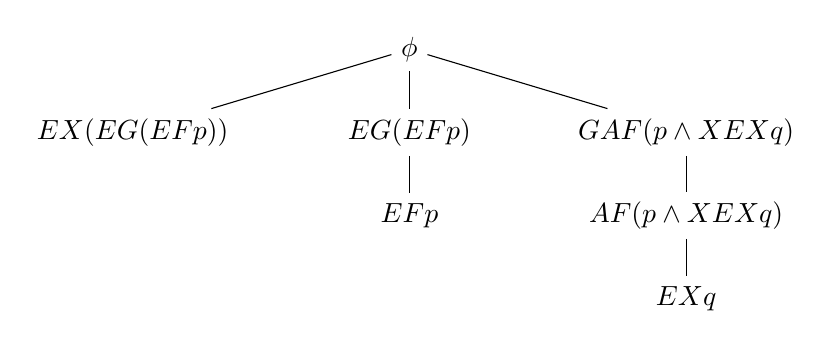
\begin{tikzpicture}[sibling distance=10em, level distance=3em]
    \node {\(\phi\)}
      child { node {\(EX(EG(EFp))\)}}
      child { node {\(EG(EFp)\)}
        child { node {\(EFp\)}}
      }
    child { node {\(GAF(p\land XEXq)\)}
      child { node {\(AF(p\land XEXq)\)}
            child { node {\(EXq\)}}
          }
        };
  \end{tikzpicture}
\end{center}

  Possiamo quindi fare questo flattening aggiungendo le atomi proposition.

\begin{center}
  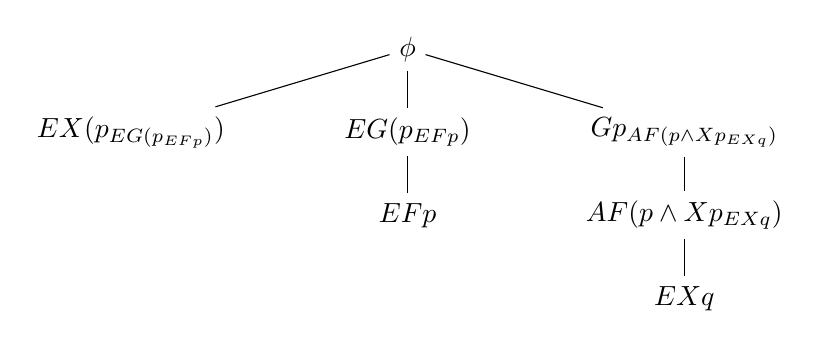
\begin{tikzpicture}[sibling distance=10em, level distance=3em]
    \node {\(\phi\)}
      child { node {\(EX(p_{EG(p_{EFp})})\)}}
      child { node {\(EG(p_{EFp})\)}
        child { node {\(EFp\)}}
      }
    child { node {\(Gp_{AF(p\land Xp_{EXq})}\)}
      child { node {\(AF(p\land Xp_{EXq})\)}
            child { node {\(EXq\)}}
          }
        };
  \end{tikzpicture}
\end{center}

Chiaramente la complessità di questo algoritmo è n volte quella di LTL, che è PSPACE\@, con \(n\) numero di sottoformule di \(CTL^*\), che è lineare nella lunghezza della formula, dunque complessità totale è ancora PSPACE\@.

Un altro modo è di usare automi ad albero, che riesce a ottenere PSPACE\@. Per quato riguarda SAT e VALIDITY, è possibile mostrare che si arriva 2EXPTIME a differenza di LTL che rimane PSPACE\@.

\(CTL^*\) però è un gran guadagno a livello di espressività. Infatti LTL è contenuto in \(CTL^*\) poiché ogni formula \(\psi\) in LTL è equivalente a \(A \psi\) in \(CTL^*\). Inoltre è stato anche dimostrato che si può verificare anche il contrario in un certo senso, ovvero data una formula \(\phi \in CTL^*\) se esista un \(\psi \in LTL\) tale che \(\phi \equiv A\psi\).

È stato mostrato infatti che presa una formula in \(CTL^*\) e eliminando banalmente tutti i quantificatori si ottiene una formula in LTL che è l'unica possibile formula LTL equivalente all'originale una volta quantificata universalmente a monte. Di conseguenza presa una qualsiasi formula \(\phi \in CTL^*\) si può facilmente produrre \(\hat{\phi} \in LTL\) eliminando i quantificatori, e poi mostrare che \(\phi \equiv A \hat{\phi}\) che è verificabile riducendo il problema a SAT della formula \(\neg ((\phi \to A \hat{\phi}) \land (A\hat{\phi} \to \phi)) \). Se questa formula è soddifacibile allora le formule non sono equivalenti, altrimenti lo sono. 

Questa idea può essere estesa anche a \(CTL\), ovvero data una formula \(\phi \in CTL\) esiste una formula \(\psi \in LTL\) tale che \(\phi \equiv A\psi\). Essendo infatti \(CTL\) un frammento di \(CTL^*\) si può appllicare banalmente l'algoritmo di cui sopra.

Un'ultima domanda è l'inversa, ovvero data \(\psi \in LTL\) esiste una formula \(\phi \in CTL\) tale che \(\psi \equiv A\phi\)? A tale domanda ad oggi non è stata data una risposta, e rimane un problema aperto.

Andiamo a vedere dunque qualche esempio di formula \(CTL^*\) non esprimibile in \(CTL\)\@.
Consideriamo \(A FGp\). Prendiamo ad esempio il modello seguente.

TODO MIGLIORA 

p -> ~p -> p (entrambi i p self loop)

L'estensione ad albero di tale modello è chiaramente

                   p
                ~p   p
               p  ~p   p
             p   p   ~p p

Chiaramente qui \(A FGp\) vale. Proviamo a vedere di trasformarla in \(CTL\). La cosa più ovvia sarebbe \(A FEGp\) oppure \(A FAGp\). Putroppo non funziona. \(A FAGp\) è falsa già nel modello di esempio, mentre \(A FEGp\) è vera nel modello dato ma esistono altri modelli per cui \(A FGp\) è vera e \(A FEGp\) no, quindi non sono equivalenti. Una possibile causa del problema è la natura esistenziale di \(F\) che cozza con \(A\).

Altro esempio è \(AF(p \land Xp)\). Anche qui, la formula più ovvia è \(AF(p \land AXp)\) ma purtroppo non è vera già nel modello di esempio perché nel percorso con soli p ogni nodo ha almeno un figlio con etichetta \(\neg p\), mentre \(AF(p \land Xp)\) è vera. Se invece consideriamo \(AF (p\land EXp)\) questa è soddisfatta dal modello

~p -> p -> ~p (2 e 3 con self loop)

la cui estensione ad albero è

                   ~p
                    p
                 ~p   p
                ~p  ~p p

Ma la formula originale non è soddifatta qui, perché ci sono percorsi in cui non ci sono mai due p consecutive.

Un ultimo esempio è con la classica fairness \(A(GFp\to Fq)\). Anche qui, la formula più ovvia è \(AG AF p \to AFq\) ma qui si vede subito che il quantificatore iniziale ha cambiato scope. In particolare in modelli che falsificherebbero l'originale possono soddisfare la seconda falsificando la premessa dell'implicazione.

Vediamo ora un esempio di proprietà \(CTL\) non esprimibile in \(LTL\). Consideriamo \(AGEFp \in CTL\). Vogliamo mostrare che non esiste \(\psi \in LTL\) tale che \(AGEFp \equiv A\psi\). Supponiamo per assurdo che esista tale \(\psi\).
Consideriamo quindi il modello k

s0 -> s1 -> s3 (self)
      ||
      s2 (self)

Se s3 è etichettata con \(p\) si ha sempre vero \(EFp\) perché s3 è sempre raggiungibile. Di conseguenza tale modello soddisfa \(AG EFp\).

Consideriamo allora il modello k' senza s3, ovvero

s0 -> s1
      ||
      s2 (self)

Qui non è mai soddisfatta p quindi non può essere soddisfatta \(EFp\) e dunque non è soddisfatta \(AG EFp\).
Ma possiamo notare che tutti i percorsi infiniti di questo secondo modello appartengono anche al primo.
Quindi essendo che \(k\models AGEFp\) allora \(k \models A\psi\) e quindi in particolare \(k\models \psi\). Ma essendo che tutti i percorsi di k' sono in k, ed essendo che le formule LTL lavorano su i percorsi abbiamo \(k' \models \psi\) e quindi \(k' \models A\psi\) e quindi \(k' \models AGEFp\), che è assurdo.

Chiudiamo con un diagramma di Venn che esemplifica la gerarchia di espressività dei linguaggi visti

TODO aggiungi diagramma 
\(CTL^*\) contiene entrambi che hanno intersezione non vuota ma non sono contenuti
A p U q è intersezione
AGEF p solo in \(CTL\)
\(AF(p \land Xp)\) solo in LTL
la loro congiunzione è solo in \(CTL^*\)

Inizio logica giochi.

\chapter{Lezione 18/05}

Parliamo di logica per strategia e concurrent game structure. Abbiamo visto l'esempio di sasso carta forbice. Ora vedremo la formalizzazione di struttura di giochi cercando di capire il perché le cose sono importanti e poi vedremo una logica per parlare di questi giochi ovvero ATL che è un ESTENZIONE di \(CTL\)\@.

\begin{definition}{Concurrent Game Structure}
  Una \keyword{concurrent game structure} è una quadrupla \(G=\langle AP, Ag, Ac,Ps, p_0 \in Ps, \delta, \lambda \rangle\) con
\begin{itemize}
  \item \(AP\) insieme di atomic proposition
  \item \(Ag\) insieme di agenti o giocatori
  \item \(Ac\) insieme di azioni che gli agenti possono compiere\footnote{In realtà è possibile anche avere un insieme di azioni per ogni agente, ma per semplicità consideriamo un unico insieme di azioni condiviso da tutti gli agenti}
  \item \(Ps\) insieme delle posizioni del gioco, analogo ai mondi o gli stati di una struttura di kripke
  \item \(p_0\) posizione iniziale
  \item \(\delta\) funzione di transizione
  \item \(\lambda: Ps \to 2^{AP}\) funzione di etichettatura
\end{itemize}

\end{definition}

Come possiamo notare, questa è molto vicina a una kripke structure che è definita come \(K=\langle AP,W,w_0 \in W,R,\lambda\rangle\) con \(AP\) insieme di atomic proposition, \(W\) insieme di stati, \(w_0 \in W\) stato iniziale, \(R \subseteq W\times W\) relazione di transizione seriale, ovvero tale che \(\forall w\exists v (w,v) \in R\), e \(\lambda: W \to 2^{AP}\) funzione di etichettatura.

La differenza principale è che \(\delta\) non è una relazione ma una funzione, perché modella l'evoluzione a valle delle azioni degli agenti. In particolare stando modellando giochi concorrenti e non a turni. Di consiguenza avremo \(\delta: Ps \times Ac^{Ag} \to Ps\) dove \(Ac^{Ag}\) è l'insieme delle funzioni che associano a ogni agente un azione. Questo insieme è quello che modella il non determinismo, poiché a differenza delle kripke structure questo è catturato dalle azioni dei giocatori.

Proviamo quindi a modellare sasso-carta-forbici. Sicuramente avremo
\begin{itemize}
  \item \(Ag = \set{1,2}\)
  \item \(Ac = \set{S,C,F}\)
  \item \(Ps = \set{p_0, p_1, p_2}\) con \(p_0\) stato iniziale in cui non c'è un vincitore, \(p_1\) stato in cui vince il giocatore 1 e \(p_2\) stato in cui vince il giocatore 2.
  \item \(p_0 = p_0\)
\end{itemize}

Le transizioni sono espresse dall'automa seguente:

AGGIUNGI AUTOMA
che è formalizzato da \(\delta\) che è definita come segue
\[\delta(p,(a_1,a_2)) = \begin{cases}
                          p_0 & \text{se } a_1 = a_2 \land p = p_0 \\
                          p_1 & \text{se } (a_1,a_2) \in \set{(S,F),(C,S),(F,C)} \land p = p_0 \\
                          p_2 & \text{se } (a_1,a_2) \in \set{(S,C),(C,F),(F,S)} \land p = p_0 \\
                          p & \text{se } p \in \set{p_1,p_2}
                        \end{cases}\]

\begin{note}
  Nonostante abbiamo formalizzato \(\delta\) come una funzione che chiede una funzione che associa agenti a azioni, rappresentando gli agenti con numeri è possibile esprimere la funzione come una tupla in cui a ogni posizione è assocciato l'agente con lo stesso numero che rappresenta l'agente che compie quell'azione. Ad esempio, \(\delta(p,(S,C))\) è equivalente a \(\delta(p, d)\) con \(d(1) = S\) e \(d(2) = C\). Tali funzioni sono dette \keyword{decisioni collettive}.
\end{note}

Questo poiché stiamo modellando sasso-carta-forbice come un gioco che si gioca una sola volta, e dunque una volta che si è arrivati in uno stato di vittoria non si esce più da quello stato.

Per quanto riguarda \(AP\) e \(\lambda\) come solito dipende dalle proprietà che vogliamo verificare. Ad esempio con \(AP = \set{{win}_1, {win}_2}\) che indicano rispettivamente se il giocatore 1 o 2 ha vinto, e con \(\lambda(p_0) = \emptyset\), \(\lambda(p_1) = \set{{win}_1}\) e \(\lambda(p_2) = \set{{win}_2}\) possiamo verificare proprietà riguardo la vittoria.

Con questo modello oltre che a giochi è possibile modellare in generale qualsiasi tipo di interazioni tra agenti che interagiscono concorrentemente nel modificare un sistema, come ad esempio processi che interagiscono in un sistema distribuito, o robot che interagiscono in un ambiente condiviso, o anche persone che interagiscono in un sistema sociale.

Inoltre, questa modellizzazione è sufficientemente generale da poter modellare anche giochi non concorrenti, ma a turni. Vediamo ad esempio il tris.

AGGIUNGI ESEMPIO INIZIALE DEL GRAFO DEGLI STATI DEL TRIS (già presente nella cartella images)

con i numeri vicino agli stati che indicano quante altre posizioni simmetricamente equivalenti ci sono.

Chiaramente qui avremo \(Ag = \set{\times, \circ}\). Dobbiamo capire come codificare le varie caselle, che in questo caso descrivono anche le azioni essendo che ogni giocatore come azione può solo riempire col proprio simbolo una casella. Possiamo ad esempio codificare le caselle con i numeri da \(1\) a \(9\). Dovremmo anche capire come codificare le azioni non permesse, che potremo modellare con una sconfitta automatica.

Venendo quindi agli stati, enumerarli tutti è molto comlicato avendo \(9\) celle con \(3\) possibili valori diversi, ovvero vuota \(\square\), \(\times\) e \(\circ\). Dunque il modo migliore per descriverlo è \(\set{\square, \times, \circ}^9\), ovvero le posizioni sono descritte da funzioni che associano a ogni cella cosa c'è dentro. Dovremmo anche aggiungere due stati per indicare una mossa errata, ovvero \(\set{\bot_{\times}, \bot_{\circ}}\) A questo punto avremo lo stato inziale rappresentato dalla funzione che associa \(\square\) a tutte le celle, ovvero \(p_o: n \to \square, \forall n \in \set{1,\dots,9}\).

Ora il vero momento in cui codifichiamo il fatto che il gioco è a turni, ovvero la funzione di transizione. In particolare dovremmo semplicemente ignorare l'azione del giocatore di cui non è il turno.
Ad esempio come prima mossa potremmo avere
\[\delta(p_0, d) = \set{p_i: *\setminus i \mapsto \square, i \mapsto \times}[ i = d(1)]\]

o ad esempio per la posizione \(5\)

\[\delta(p_5, d) = \begin{cases}
  p_{5i}: * \setminus \set{5,i} \mapsto \square, 5 \mapsto \times, i \mapsto \circ & ,d(2) = i \\
\end{cases}\]

Questo modello ci viene utile rispetto alle strutture di kripke, poiché tali strutture modellano tutto ciò che non è il sistema come un unica entità inglobata dal non determinismo. Questo tipo di struttura ci fornisce più granularità, potendo modellare ogni entità che interagisce nel sistema in modo autonomo e quinid carattarizzare comportamenti antagonisti, colaborativi o un mix delle due.

Ci serve adesso un linguaggio per parlare di proprietà di questo sistema, e quindi andremo a introdurre una logica estensione di \(CTL\) e \(CTL^*\).

Vedremo la logica \(ATL\) e \(ATL^*\), ovvero Alternating-time temporal logic.

Queste logiche si basano su macchine alternati, ovvero a differenza delle macchine non deterministiche che richiedono l'esistenza di run accettanti, o delle macchine universali che richiedono che ogni run accetti, qui si dovrà avere un alternanza di esistenzialità e universalità.

\begin{definition}{\(ATL^*\)}
  \[\phi := p \mid \neg \phi \mid \phi \land \phi \mid \phi \lor \phi \mid \GDia[A]\psi \mid \GBox[A] \psi\]
  \[\psi := \phi \mid \neg \psi \mid \psi \land \psi \mid \psi \lor \psi \mid X\psi \mid \psi U\psi \mid \psi R \psi\]

  Con \(A \subseteq Ag\). Intuitivamente si ha
  \begin{itemize}
    \item \(\GDia[A] \psi\) è vera se esiste una strategia \(\sigma^+\) per i giocatori di \(A\) tale che, per ogni strategia \(\sigma^-\) di \(Ag\setminus A\) tale che \(\pi\models \psi\) con \(\pi\) è il percorso identificato dalla coppia \(\sigma^+, \sigma^-\)
    \item \(\GBox[A] \psi\) è vera se per ogni strategia \(\sigma^+\) per i giocatori di \(A\) esiste una strategia \(\sigma^-\) di \(Ag\setminus A\) tale che \(\pi\models \psi\) con \(\pi\) è il percorso identificato dalla coppia \(\sigma^+, \sigma^-\)
  \end{itemize}

  In un certo senso \(\GDia \psi\) è una generalizzazione di \(E\psi\) e \(\GBox \psi\) è una generalizzazione di \(A\psi\) per giochi a un giocatore, dove \(Ag = A = \set{1}\) e \(Ag\setminus A = \emptyset\).
\end{definition}

\begin{definition}{\(ATL^*\)}
  \[\phi := p \mid \neg \phi \mid \phi \land \phi \mid \phi \lor \phi \mid \GDia[A]\psi \mid \GBox[A] \psi\]
  \[\psi := \phi \mid X\psi \mid \psi U\psi \mid \psi R \psi\]


\end{definition}

Tali definizioni sono ancora informali, ma possiamo già notare che questi operatori son duali, nel senso che \(\neg \GDia[A]\psi \equiv \GBox[A] \neg \psi\)

Dobbiamo andare quindi a formalizzare il concetto di strategia e di percorso in una concurrent game structure.

Partendo da percorso, avremo che \(\pi \in Path(G) \subseteq Ps^\omega\) se \(\forall i \in [0,\abs{\pi}-1). \exists d \in Ac^{Ag}. \pi_{i+1} = \delta(\pi_i,d)\). Il che è equivalente a vedere i percorsi nella struttura di kripke sottostante. Alcuni percorsi però possono dipendere dalla sotria delle decisioni prese dai giocatori.

Questo in realtà è un problema che c'era anche nelle strutture di kripke e nelle logiche temporali. Prendiamo ad esempio la struttura

AGGIUNGI FOTO GIAÀ PRESENTE NELLA CARTELLA IMAGES

Chiaramente questa struttura verifica \(F(p\land Fq)\). Ma per farlo è necessario fare scelte diverse in \(w_0\), e quindi devo ricordarmi delle scelte passate per fare quelle giuste. Se facessi scelte guardado solo lo stato attuale non sarei in grado di soddisfarle. In reltà si dimostra che se non ci fosse memoria potrei verificare solo percorsi lasso, ovvero con la forma:

AGGIUNGI IMMAGINE

Si dimostra però che per avere proprietà per cui è indispensabile la memoria mi serve innestare operatori temporali, e quindi rimanendo in \(CTL\) o in ATL la memoria non sarà necessaria.

A questo punto però è necessario anche il concetto di storia:

\[Hst = \set{\pi \in Path(G)}[\abs{\pi} < \omega]\]

Possiamo quindi definire una strategia come
\[\sigma: Hst \to Ac\]

Ovvero una funzione che associa a ogni posizione della storia una azione, intuitivamente quella che è stata presa nella posizione.
Ovviamente una trategia per un insieme di giocatori \(A\subseteq Ag\) sarà \(\set{\sigma_a}_{a \in A}\), ovvero una sequenza di strategie per ogni giovatore.

Una coppia di strategie di gruppi di giocatori tali che l'unione dei gruppi è \(Ag\) è detta \(play\):
\[\pi = play(\sigma_A,\sigma_{Ag\setminus A}) \in Path(G,p_0)\]
tale che \(\pi\) è coerente con le scelte fatte dai giocatori nelle strategie \(\sigma_A\) e \(\sigma_{Ag\setminus A}\), ovvero

\[\forall i \in \N, \pi_{i+1} = \delta(\pi_i, d_i)\]
con
\[d_i(a) = \begin{cases}
  \sigma_A^a(\pi_{\leq i}) & a \in A \\
  \sigma_{Ag\setminus A}^a(\pi_{\leq i}) & a \in Ag\setminus A
\end{cases}\]

Ovvero a ogni passo \(i\) la posizione successiva è determinata dalle azioni scelte dai giocatori in quel passo, che sono determinate dalle strategie che dipendono dalla storia fino a quel punto.

Noi ci concentreremo essenzialmente su ATL poiché ha la proprietà di poter essere soddisfatta da strategie memoryless, ovvero in cui una strategia è esclusivamente \(\sigma: Ps\to Ac\) ovvero solo l'ultimo stato conta. Non vedremo la dimostrazione, ma idealmente si può mostrare che se una formula è soddisfatta da percorsi con cicli non semplici posso sempre eliminare i cicli non semplici accorpandoli in un unico ciclo semplice che mi crea la struttura a lasso.

Essendo che le strategie memoryless di fatto identificano degli archi avremo che un play identifica un sottografo, in cui mantengo solo gli archi effettivamente percorsi. Tra l'altro tale grafo è deterministico, ovvero partendo dallo stato inziale esiste un solo percorso.

A questo punto per verificare prorietà sarà sufficiente verificare la raggiungibilità su i vari sottografi indotti.

Essendo che gli operatori \(\GDia\) e \(\GBox\) nascondono internamente una quantificazione alternata (\(\forall\exists, \exists\forall\)) non è possibile in \(CTL\) esprimere tutto ciò che è esprimibile in ATL. In particolare \(CTL\) è semanticamente un frammento di ATL in cui scelgo solo coalizioni \(A=\emptyset\) o \(A = Ag\) rendendo vacuo un quantificatore.

Inoltre abbiamo visto che in \(CTL\) erano vere proprietà di one-step unfolding, ovvero

\[A/E \phi_1 U \phi_2 \equiv \phi_2 \lor (A/E \phi_1 \land A/E X(A/E \phi_1 U \phi_2))\]
\[A/E \phi_1 R \phi_2 \equiv \phi_2 \land (A/E \phi_1 \lor A/E X(A/E \phi_1 R \phi_2))\]

Inoltre osservando che queste proprietà è di punto fisso abbiamo potuto riscriverla come \(E \phi_1 U \phi_2 \equiv \mu V. \phi_2 \lor (\phi_1 \land EX V)\) e \(E \phi_1 R \phi_2 \equiv \nu V. \phi_2 \land (\phi_1 \lor EX V)\) da cui abbiamo estratto gli algoritmi di model checking. Anche in ATL sono presenti delle equazioni di punto fisso identiche. Di conseguenza l'unica cosa che dovremo cambiare per il model checking sarà solo l'operatore pre, che sarà più complicato dovendo cogliere l'alternanza.

\chapter{Lezione 25/05}

La struttura di kripe indotta da una concurrent game structure è essenzialmente la stessa con \(R\) tale che \((s_1,s_2) \in R\) se e solo se \(\exists d \in Ac^{Ag}. s_2 = \delta(s_1,d)\). Questo giustifica il vedere ATL come estensione di \(CTL\) e in particolare vedere gli operatori \(\GDia\) e \(\GBox\) come generalizzazioni di \(E\) e \(A\). Nella terminologia dei giochi l'insieme di agenti vengono dette coalizioni. Quindi \(\GDia[A] \psi\) ci diche che esiste una stategia per la coalizione \(A\) tale che ogni strategia della coalizione complementare \(\overline{A}\) verificano \(\psi\) e dualmente per \(\GBox\).

Abbiamo quindi formalizzato il concetto di strategia analizzando il fatto che tali strategie dipendono dalla storia. Noi ci concentreremo solo sulle strategie memoryless.

Possiamo definire quindi in modo più preciso la semantica degli operatori \(\GDia\) e \(\GBox\) in ATL\@.

\[G,s\models \GDia[A] \psi \text{ se } \exists \sigma_A \in Str(A) \forall \sigma_{\overline{A}} \in Str(\overline{A}). G,s,play(\sigma_A,\sigma_{\overline{A}})\models \psi \]

Si vede facilmente che l'unica differenza rispetto a \(CTL\) è la quantificazione sulle strategie degli avversari. Se infatti consideriamo \(\GDia[Ag] \psi\) allora \(\overline{A} = \emptyset\) e quindi \(\GDia[Ag] \psi\equiv E\psi\). Il verso \(\implies\) è banale, mentre per quello inverso basta prendere il percorso che soddisfa \(E\psi\) e costruire per ogni passo la strategia adeguata, non essendoci una coalizione antagonista.

\[G,s\models \GBox[A] \psi \text{ se } \forall \sigma_A \in Str(A) \exists \sigma_{\overline{A}} \in Str(\overline{A}). G,s,play(\sigma_A,\sigma_{\overline{A}})\models \psi \]

Ovvviamente si ha \(\GBox[Ag] \psi \equiv A\psi\) con dimostrazione simile a quella precedente. Quindi \(CTL\) equivale a ATL con la \keyword{grand coalition}, ovvero una coalizione di tutti gli agenti. Dunque ATL è più espressiva.

Prendendo l'esempio di carta sasso forbice possiamo dire che esistono weak strategy, ovvero per ogni agente c'è una strategia dell'altro che lo avvantaggia. Formalmente
\[\GBox[\set{1}] F s_1\land \GBox[\set{2}] F s_2\]
Ma non ci sono strategie vincenti
\[\neg \GDia[\set{1}] F s_1 \land \neg \GDia[\set{2}] F s_2\]

ATL non ha bisogno di memoria, nel senso che le proprietà che richiedono memoria non sono esprimibili in ATL.

Per fare l'algoritmo di Model checing \(CTL\) abbiamo sfruttato il one-step unfolding che ci ha permesso di costruire una funzione monotona e quindi sfruttare una costruzione a punto fisso. Cerchiamo di farlo anche per ATL.

In particolare abbiamo visto
\[E \phi_1 U\phi_2 \equiv \phi_2 \lor (\phi_1\land E X E \phi_1 U\phi_2)\]

Dobbiamo mostrare che valga
\[\GDia[A] \phi_1 U\phi_2 \equiv \phi_2 \lor (\phi_1\land \GDia[A] X \GDia[A] \phi_1 U\phi_2)\]

È facile vedere che \(\GDia[A] \phi_1 U\phi_2 \equiv \phi_2 \lor (\phi_1\land \GDia[A] X \phi_1 U\phi_2)\) perché è sufficiente prendere la strategia che rende vera la formula che assumo vera e usarla per l'altra e si vede facilmente che va bene pure per l'altra. La parte difficile è nello spezzare gli operatori temporali. In \(CTL\) quando spezzavamo un percorso era facile perché il next non era altro che prendere il primo e poi il resto. Adesso abbiamo un alternanza di quantificatori in principio e quindi la scelta di una strategia scelta aprioristicamente che mi assicura \(U\) per quanto riguarda \(GDia[A] X \phi_1 U\phi_2\). Nello spezzare in \(\GDia[A] X \GDia[A] \phi_1 U\phi_2\) invece mette su una doppia alternanza perché la semantica è

\[\exists \sigma_A \forall \sigma_{\overline{A}} \exists \sigma_{A}' \forall \sigma_{\overline{A}}' play(\sigma_{A}',\sigma_{\overline{A}}',{\left(play(\sigma_A,\sigma_{\overline{A}},s)\right)}_1) \]

Quello che vorremmo mostrare è che questa alternanza è irrilevante, e che bastano i primi due quantificatori. Una perima versione per i giochi a somma zero finiti il cui goal è un istanza di reachability è stato dimostrato da Zermelo che è sempre vero che almeno un giocatore ha una strategia vincente.

\[\exists \sigma_1 \forall \sigma_2 Win_1(\sigma_1,\sigma_2) \lor \exists \sigma_2 \forall \sigma_1 Win_2(\sigma_1,\sigma_2) \]

Nel prim'ordine questa struttura è falsificabile da un qualsiasi modello a grafo che non ha ne oggetti iniziali ne terminali. Ma per i giochi finiti a somma zero questo è sempre verificato. Questo in oltre vale solo per i giochi a turni.

Un modo per mostrare quindi che si può spezzare creando un gioco a somma zero tra un verificatore e un rifiutatore della formula e sfruttare il teorema di zermelo per mostrare che almeno uno dei due ha una strategia vincente. 

Un altro modo è costruttivo, usando le strategie della formula che assumo vera per costruire quelle della formula che voglio mostrare equivalente. Se ad esempio vogliamo mostrare \(\GDia[A] X \phi_1 U\phi_2 \implies \GDia[A] X \GDia[A] \phi_1 U\phi_2\) posso usare la strategia del primo per copiarla per la seconda, e mostrare che va bene. Nell'altro verso invece ne ho due, allora uso quella del next per fare il per togliere il primo stato dalla history e poi quella dell'until appropriato rispetto al risultato della strategia del next per il resto. Si passa quindi da strategie senza memoria a temporaneamente strategia con memoria che posso sempre riportare a memoria zero.

Funziona uguale per il release:

\[\GDia[A] \phi_1 R \phi_2 \equiv \phi_2 \land (\phi_1 \lor \GDia[A] X \GDia[A] \phi_1 R\phi_2)\]

A differenza di CTL non potremo passare al \(G\) perché questa formula non distribuisce
\[\GDia[A] \phi_1 R \phi_2 \equiv \GDia[A] ((\phi_2 U (\phi_2 \land \phi_2)) \lor G \phi_2)\]

In ogni caso però con la stessa identica dimostrazione vista per CTL questi sono ancora rispettivamente minimo e massimo punto fisso. L'unica differenza è che dovremo fare induzione completa su un albero di percorsi piuttosto che induzione lineare su un singolo percorso.

Quindi quello che ci rimane è l'operatore \(X\) o equivalentemente nella forma denotazionale la funzione \(pre\). Questa è la grande sostanziale differenza, poiché avendo più giocatori il concetto di preimmagine è più complesso. Prima infatti \(pre\) catturava \(EX\), ma ora dobbiamo fare \(\GDia[A]X\). Nella semantica dovremmo lavorare sulle strategie, ma essendo che stiamo lavorando con \(X\) ci interessa solo un passo, e quindi ci interessa delle due strategie solo l'azione dato lo stato di partenza. Quindi
\[\exists \sigma_A \forall \sigma_{\overline{A}} play(\sigma_A,\sigma_{\overline{A}},s) \models X\phi \]
diventa
\[\exists {ac}_{A} \forall {ac}_{\overline{A}} \delta(s, ({ac}_A, {ac}_{\overline{A}})) \models \phi\]

Ora la definizone matematica di \(pre\) era
\[pre(V) = \set{w\in W}[\exists w' \in V. (w,w') \in R]\]

Ora però c'è un universale da trattare quindi dovremo aggioranare a 
\[pre_A(V) = \set{w\in W}[\exists {ac}_{A} \in Ac^A \forall {ac}_{\overline{A}} \in Ac^{\overline{A}}. \delta(w, ({ac}_A, {ac}_{\overline{A}})) \in V]\]

Essendo che a livello algoritmico l'unica cosa usata di fatto è il punto fisso (che rimane uguale) e il \(pre\) ci basta per il model checking cambiare il \(pre\) di CTL con questa versione più a grana fine.

Questo algoritmo rimane polinomiale sugli archi, ma purtroppo questo algoritmo è esponenziale nei giocatori, poiché per ogni stato e ogni azione della coalizione \(A\) devo verificare tutte le azioni della coalizione complementare \(\overline{A}\). In generale però se il numero di giocatori è piccolo, o se le azioni sono limitate, questo algoritmo è comunque efficiente.
